\section{Introduction}
\label{sec:introduction}

The Internet has evolved enormously since its inception. From just a simple communication layer for information sharing between researchers, it has grown into a ubiquitous platform for every user and any use. 
A flurry of organic changes to its infrastructure and interfaces has accompanied this vast transformation.

% The pooling and sharing of compute and networking capabilities and their provisioning as a service, known as the Cloud Computing paradigm, has given individuals and enterprises alike access to practically unlimited amounts of virtualised resource components. 
In a little over a decade of existence over the Internet, the Cloud has earned users tremendous benefits by rendering virtually unlimited quantities of computing resources available in an affordable, fit-for-purpose, and rapidly scalable manner.
% The massive success of the Cloud, however, has also highlighted important deficiencies in the nature of its architecture: the huge energy footprint of its (immense) data centres; the intrinsic vulnerability to single-point failure of its centralised model; the latency caused by storing and processing in the Cloud all the data ingested at the periphery of it (allusively called the Edge); the threats to data security and privacy incurred by exposing sensitive data to Edge-Cloud transfers.

Similarly, dramatic improvements in mobile connectivity occurred in the last two decades in terms of ubiquity, reliability, and affordability, have allowed anyone to access the Internet from anywhere and at any time.
% The massive boost and evolution of mobile computing, which has led to the emergence of richer client-side web apps, is expected to grow further with the uptake of 5G connectivity~\cite{ericsson-5g}. The consequent impetuous growth of the Internet of Things is predicted to grow exponentially in the coming years~\cite{gartner-iot}.
Commercial forecasts predict that by the end of 2028, over 5 billion people, over $60$/\% per cent of the world population, will have a 5G coverage subscription~\cite{ericsson-5g}, with everyday objects connected to the Internet and to each other. 
As such "things" comprise a multitude of heterogeneous devices ranging from consumer devices, like mobile phones and wearables, to industrial sensors and actuators~\cite{chen2018edge}, this step of evolution has given exponential growth of the Internet of Things (IoT), which spans smart transportation systems, grids~\cite{mugarza2019dynamic}, and even cities \cite{cabrini2021enabling}.
%(represented on the right in Figure~\ref{fig:continuum}).
% The consequent impetuous growth of the Internet of Things, with the number of connected devices predicted to grow exponentially in the coming years~\cite{gartner-iot}, makes Cloud centralisation increasingly less practical~\cite{mell2011nist}.
%As a consequence of connecting "things" to the Internet, large masses of data are being generated at unprecedented volumes, variety and velocity. 
%\textcolor{red}{In the traditional (and na\"ive) centralised model, such data is transferred and stored in the centre of Cloud.
%Data transfer, especially at these volumes, is costly in networking pricing (e.g. ingress traffic to the Cloud and transportation) and delays actual computation.}
%It is therefore apparent that traditional data processing methods where data is collected at the Edge and processed centrally is not sustainable. 

In this arrangement, a more decentralised solution is required. The Continuum is a collective infrastructure where data processing may take place dynamically where it is deemed most convenient under any of the criteria of interest (latency, privacy, energy, etc.). The concept enables the traditional Internet and the Internet of Things to integrate into a seamless Continuum, where a multitude of as-a-service applications may be developed, deployed, and employed regardless of location~\cite{beckman2020harnessing}. The Cloud and the Edge can both benefit from forming the Continuum together, allowing Cloud-alike virtualized access to the physical world to occur in a more distributed and dynamic manner, and favouring the creation of numerous novel latency-free, private and secure, energy-savvy services.

This vision of seamless integration extends the view in literature which regards the Cloud and the IoT as distinct spaces, with the latter sending data and offloading computation to the former but not vice versa. Likewise, the concept goes beyond merely connecting network nodes to allow computation to happen at predetermined locations in the computing space. For instance, highly dynamic scenarios comprised of mobile users and diverse applications require flexible placement of data and computing for each mobile user. Figure~\ref{fig:continuum} attempts to capture said vision pictorially. 

\begin{figure}[ht]
\centering
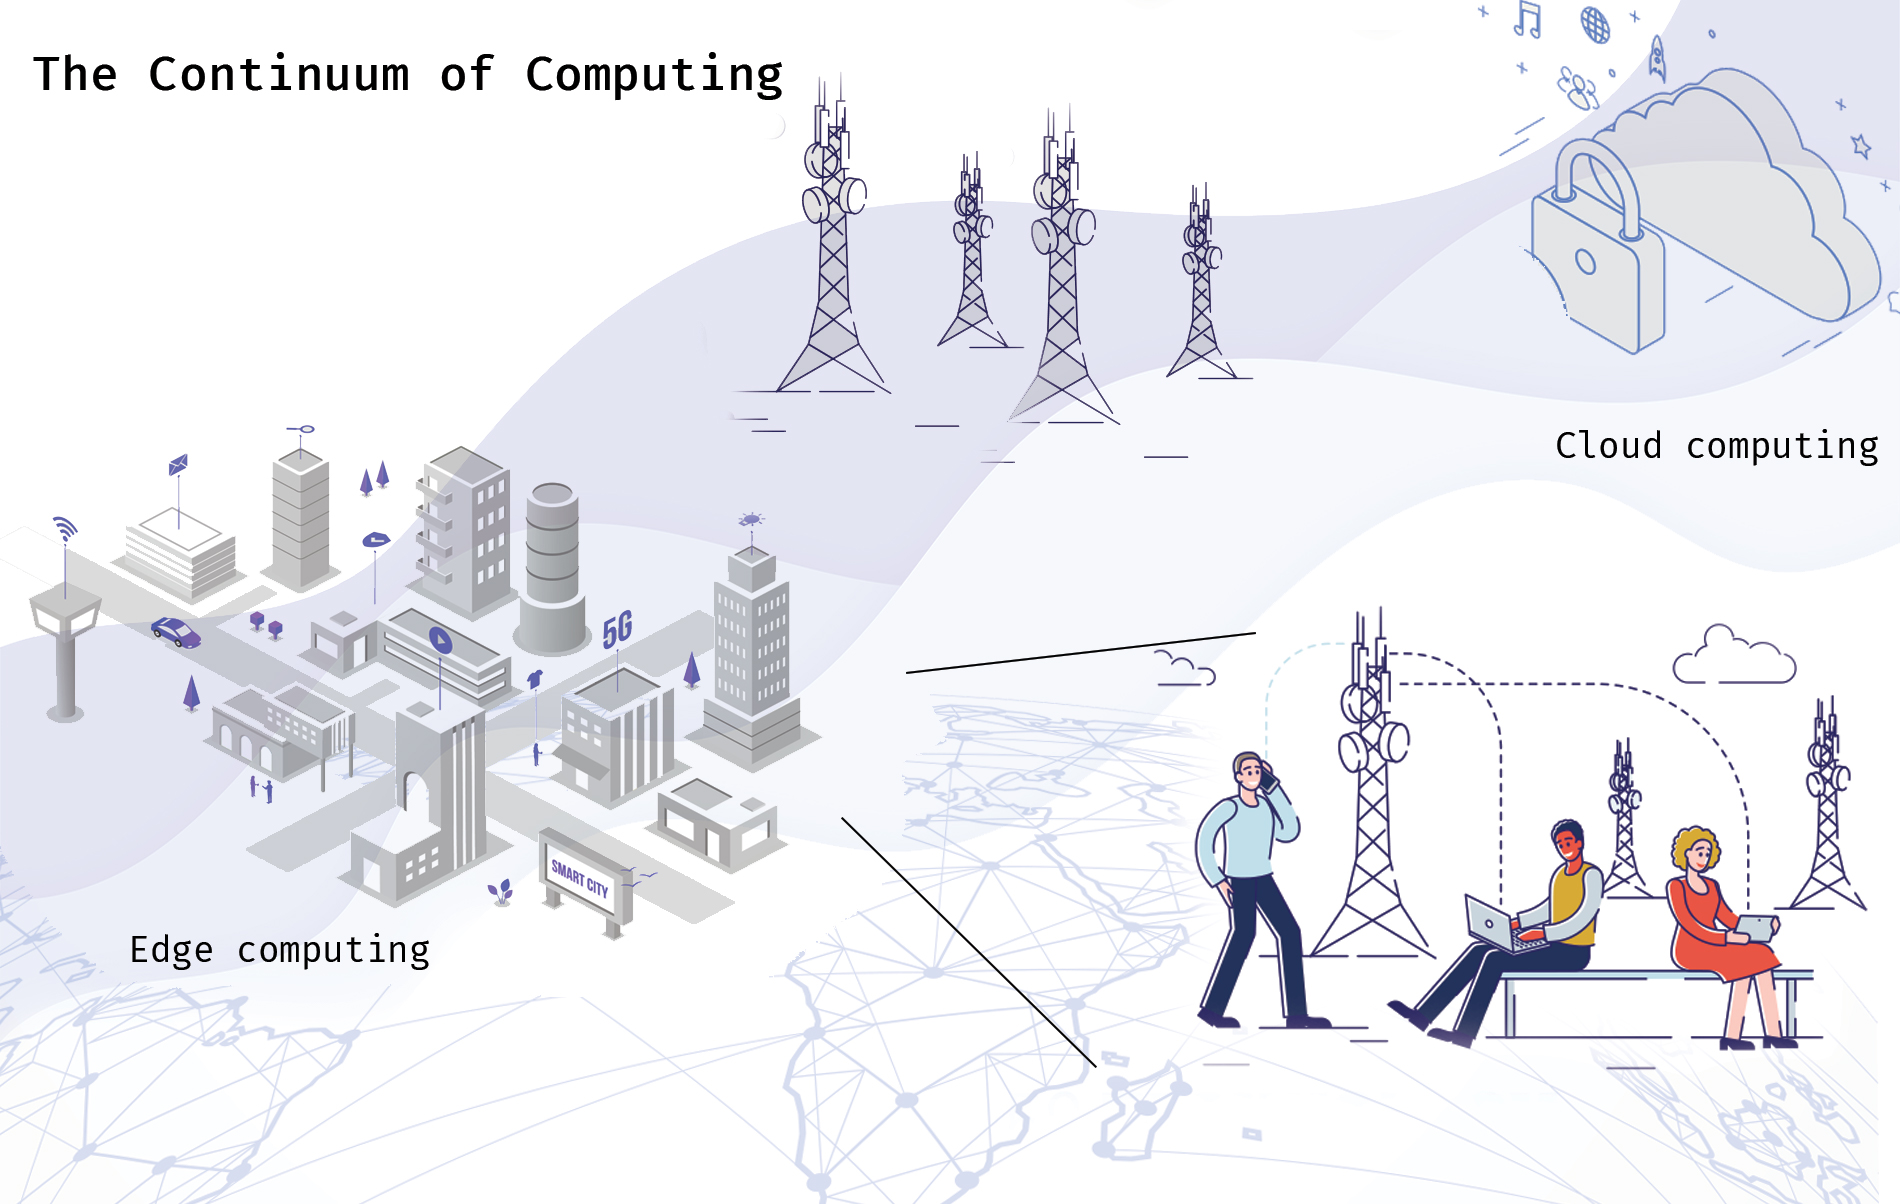
\includegraphics[width=0.7\textwidth]{figures/continuum}
\caption{Pictorial view of the Continuum of Computing comprising the Edge and Cloud computing. The Edge of the network is where physical reality begins, contrarily to the Cloud where the digital components dominate.}
\label{fig:continuum}
\end{figure}
% Enacting this vision requires that sufficient compute capabilities are deployed at the Edge of the network, where physical reality begins and connected Edge devices operate as the bridge between the physical and the digital worlds.

%\textcolor{red}{Fog computing~\cite{fog-computing} is the term coined by the research community to identify computational resources situated at a few, usually one, hop away from end users. Figure~\ref{fig: Continuum} depicts Fog nodes as base stations, which users connect to in everyday activities.}
%This paper puts forward a vision that follows naturally from the previous premises - the \textbf{Continuum of Computing} - a ubiquitous platform where distributed on-demand resources and services on the whole computing continuum are dynamically provisioned to support different ranging services and released with minimal management effort.

The foundation of the Continuum is made up of pervasive service platforms located anywhere the user is and a multitude of services, with different granularity, available over the Internet and composed opportunistically according to user needs.
%The service providers offer services, and consumers use them to accomplish any high-level application-specific goal. Services should be composed of other existing services, leveraging the principle of reuse. These services' granularity can be very different, ranging from high-level business to low-level sensing provided by the Internet of Things.
%\textcolor{red}{In essence, the Continuum is constituted by software and hardware resources provided as-a-service, which can be delivered anywhere the user is, independent of their respective location. }
% The Continuum must afford elastic provisioning of the end-to-end service delivery infrastructures virtualised to allow scaling as a function of user demand and service requirements. 

%The notion of Continuum of Computing is not entirely novel: the authors of~\cite{latre2014fluid} did envision a Fluid Internet, which "seamlessly provisions virtualised infrastructure capabilities, adapting the delivery substrate to the dynamic requirements of services and users, much like a fluid adapting to fit its surroundings". 
%This vision In a similar vein, the authors of~\cite{abdelbaky2017computing} present the notion of computing in the Continuum as "a fluid ecosystem where distributed resources and services are programmatically aggregated on-demand to support emerging data-driven application workflows". 
%Likewise, the authors of~\cite{beckman2020harnessing} define the Continuum of Computing and seek to develop approaches that include it into a collective whole.

\paragraph{Contribution}

The concept of Continuum is not entirely novel, as other authors have already described a similar vision in the past years~\cite{balouek2019towards, beckman2020harnessing}. Other researchers, such as~\cite{abdelbaky2017computing} and \cite{balouek2019towards}, have also proposed analogous visions and architectures for the Continuum, although limited to the innovation of data-driven applications. Even more interestingly, the authors of \cite{risco2021serverless} have argued the practicality of adopting the Serverless paradigm~\cite{shafiei2022serverless} for the Continuum. All the mentioned authors fall short in supporting a wide variety of applications, e.g. like long-running industrial control loops or even just mainstream Web application servers. It is, however, crucial to consider the diversity of applications from the very first stages as many aspects, like orchestration, are highly sensitive to applications and infrastructure characteristics.

On the contrary, our efforts explore the adoption of open-source technologies for building a system for the Continuum that is application-agnostic and exhibits richer characteristics such as data locality and computational mobility. Our work comprises a proposition of a reference architecture for the Continuum (Section \ref{sec:technicals}), an in-depth analysis of the problem space (Section \ref{sec:challenges}) and a  Proof of Concept that adapts and integrates various state-of-the-art technologies (Section \ref{sec:technology-selection}). We adapted well-known tools in the Cloud community and technologies still at an early stage of development to gauge the distance between the Continuum vision and its actual fruition. The result of our work and the utilised tools are open-sourced and vendor-neutral, an important step forward in easing the development of future researches in the Continuum field.

To the best of our knowledge, the adaptation and integration of open-source tools have only been assumed to be possible~\cite{menetrey2022webassembly}, without exploring how far this was actually true in practice. 

We first explored the feasibility of adapting mature Cloud-native tools like the Kubernetes~\cite{kubernetes} orchestrator to span over the whole Cloud-Edge Continuum. Notably, we explored the discoverability of Edge nodes in a Kubernetes cluster and the ubiquitous interoperability of web services. We also thoroughly experimented with integrating the nascent sandboxing standard WebAssembly~\cite{haas2017bringing} to bring container-like virtualisation and portability on comparatively powerful machines and constrained devices. 

Our experiments show that many of today's technologies fit rather well, in principle, our vision of the Continuum. We take this as a sign of convergence in the organic evolution trends of Cloud, Edge and Web. There is still, however, a substantial gap in terms of viability. On the one hand, existing production-grade tools are still figuring out how to align their Cloud-centric interface to modern use cases like Edge computing. On the other hand, nascent solutions like WebAssembly are very promising on paper in terms of designs and features but still in a state of infancy in terms of practicality. More in-depth analysis of WebAssembly is outlined in Section \ref{sec:wasm}.

% Good illustrations of such points are the pooor performance of interpreted WebAssembly in constrained devices and the lack of a standard networking WebAssembly interface, which hinder the practicality of any high-level service other than pure computation machine learning.

\section{Related Work}

\subsection{Continuum of Computing}

The work in~\cite{lynn2020cloud} provides a more comprehensive view of the trend towards integrating Cloud and IoT in a Continuum and it discusses the vision under many aspects, such as architecture, orchestration, privacy and business value. Alternatively, the researchers in~\cite{santos2021towards} and~\cite{BITTENCOURT2018134} offer a similar broad literature review regarding integrating the Edge and Cloud in a Continuum. Our work is more limited in terms of analysis of the challenges, as we restricted ourselves to those related to the presented architecture and technologies. In turn, we offer a reference architecture and a technology selection that are missing in today's literature.

Other researchers have also proposed architectures for the Continuum, but their efforts were concentrated to the idea of supporting data-driven applications~\cite{risco2021serverless, balouek2019towards, abdelbaky2017computing}. While the magnitude of data produced by the Edge is undoubtedly a key force in driving towards data-driven workflows, the Continuum vision should be expanded to a broader audience of application types. Besides, while the mentioned researches achieve the integration of Edge and Cloud in some form, they typically fail to consider the need for service composition, uniform interfaces and portabille execution throughout the Continuum. Addressing these challenges is fundamental to enable pervasive applications that present greater context-awareness and mobility.

It is also worth mentioning that the Continuum of Computing is an emerging paradigm that has been proposed by the European HiPEAC (High Performance Embedded Architecture and Compilation) Commision as well and actively promoted in its Vision for the last five years \cite{hipeac}.

\subsection{Osmotic Computing}

Back in 2014, the authors of~\cite{latre2014fluid} described the concept of Fluid Internet. This novel paradigm would seamlessly provision virtualised infrastructure capabilities based on the requirements of services and users, much like a fluid adapting to fit its surroundings. In a similar chemistry analogy, a few years later, in 2016, the authors of~\cite{villari2016osmotic} presented the vision for Osmotic Computing. Their work describes a paradigm that enables the automatic deployment of (micro)services composed and interconnected over both edge and cloud infrastructures.

Both paradigms present strong affinities to the goals and challenges of the Continuum. Notably, the Osmotic paradigm envisions the same bidirectional flow of microservices from the Cloud to Edge - and vice versa - depending on the application configuration. The difference between Osmotic Computing and the Continuum of Computing is subtle but critical in terms of the novelty of the final applications they enable, respectively.

First, Osmotic Computing involves deploying microservices, a mere evolution of today's practice of building software in silos. Instead of running the entire application in the Cloud, Osmotic Computing decomposes it into microservices and deploys the latter across cloud and edge data centres. However, such microservices are not composed of services provided by a ubiquitous intermediary service platform. Osmotic services are thus limited in their context awareness, as services like city sensors are not available, decreasing the business opportunities. Applications are built instead, at best, in numerous silos~\cite{CAMERO201984}. Indeed, the main types of microservices that the osmotic computing framework orchestrates are general-purpose microservices~\cite{villari2016osmotic}.

Second, there is a difference in semantics. Osmotic computing envisions an opportunistic \textit{balancing} of microservices between the Cloud and the Edge, whereas the Continuum emphasises a wider \textit{continuity} in terms of computing. Such continuity spans from the Cloud to the extreme Edge with highly constrained devices, all seamlessly integrated into the Continuum service platform. In contrast, Osmotic Computing limits itself to comparatively powerful machines such as Raspberry Pi. For such reasons, we emphasise the importance of exploring virtualisation technologies to truly include constrained IoT nodes as active actors in the Continuum. On the contrary, the Osmotic Computing literature focuses on more resource-demanding container-based approaches.

Third, once deployed, the Osmotic microservices are relatively stationary to the deployment location, whereas the Continuum exhibits greater levels of mobility. In case of unavailability of resources at edge/cloud, Osmotic Computing relies on solutions like message brokers (e.g. Apache Kafka) to store messages temporarily in a queued manner and resume services when the resources are available~\cite{neha2022systematic}. Contrarily, the Continuum paradigm expects the computing to temporarily fall back to the closest available location. Additionally, applications in the Continuum can move geographically to accommodate the user's movement, thanks to the seamless and ubiquitous service platform.

\subsection{Serverless Computing}

The Serverless paradigm \cite{shafiei2022serverless}, which focuses on the provision of computational functions, may seem to fit well with the premises of the Continuum. First, the Serverless programming model makes developing, deploying, and managing applications dramatically less burdensome than conventional styles.
Second, individual functions may flexibly and equally run on the Edge or the Cloud, thus earning much portability. Furthermore, the current state of technologies we later present, like WebAssembly, seems to play well with the premises of Serverless, with limited resource access. Several works from the research and industry community are actively exploring the combination of WebAssembly and Serverless Edge functions with notable results \cite{gadepalli2020sledge, hall2019execution, shillaker2020faasm}. Their work combined to the definition of serverless workflows described in \cite{risco2021serverless} offer an intriguing proposition for the Continuum.

However, while well suited for event-driven and request-reply applications, the Serverless computing model falls short for long-running services that must feature high availability and low latency, such as industrial monitoring control loops. Provisioning and instantiating a Serverless function inevitably incur additional latency due to cold start and package download, even more in the context of unpredictable mobile user patterns and distributed networks. Other authors have also proved that it can be difficult to modify stateful applications to the Serverless paradigm, e.g. conventional web servers, since the state is not easily shared among functions~\cite{MALAWSKI2020502}.

Finally, the Serverless paradigm typically requires limited execution time, limited resource access and limited specialised hardware. While these constraints enable greater scalability and mobility, it is an additional severe limitation to the scope of applications which can be deployed in the Continuum. While recent works are reducing such limitations by quickly co-locating functions in the same machine and safely sharing memory regions using the WebAssembly sandboxing \cite{shillaker2020faasm}, we deem the limitations intrinsic with the nature of the Serverless model. 

The Continuum and the Serverless models are not thus one form of computing supplanting the other. On the contrary, analogously to how the growth of general-purpose container orchestration platforms like Kubernetes was necessary to pave the way for implementing Serverless platforms, we expect a similar direction for the Continuum and the Serverless. As the Edge and the Cloud become more integrated, the Serverless paradigm will act as the dominant service delivery model \textit{within} the Continuum.

\section{A system-level view of the Continuum}
\label{sec:technicals}

\subsection{Preamble}
Highly distributed networks are the most effective architecture for the Continuum, particularly as services become more complex and more bandwidth-hungry. Although often perceived as a single entity, the Internet is actually composed of a variety of different networks. 
The net result of such articulation is that content generated at the Edge may have to traverse multiple networks, crossing peering points before reaching its destination data centre, at the centre of the Cloud, as depicted in Figure~\ref{fig:traceroute}.

\begin{figure}[ht]
\centering
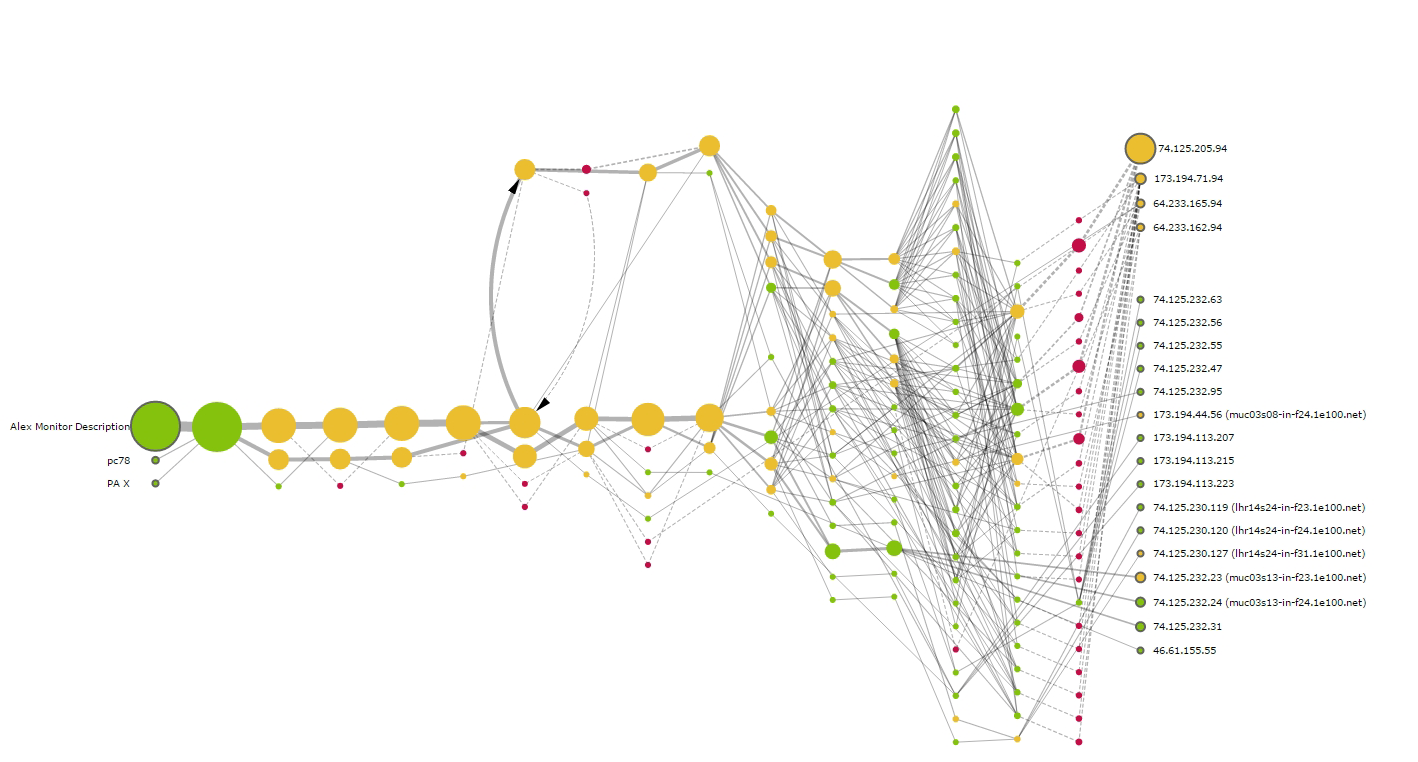
\includegraphics[width=\columnwidth]{figures/traceroute}
\caption{Traceroute virtualisation of an IP packet reaching google.com. The left green nodes are the source nodes, while packets travel across to the extreme right to servers located in data centers. Source \cite{traceroute}.}
\label{fig:traceroute}
\end{figure}

% The peering points, depicted as nodes in Figure~\ref{fig:traceroute}, where networks exchange traffic, are the common bottleneck of the Internet. Capacity at these points typically lags behind the reliability demand mainly due to the economic structure of the Internet~\cite{nygren2010akamai}. The economic incentive ramps at the first and the last mile of the source-to-destination path (Cloud data centres and IoT nodes, respectively), with very little interest attached to investing in peering points, which consequently become the cause for packet loss and increased latency.

%\textcolor{red}{Across the Internet, outages happen all the time, caused by a variety of reasons such as cable cuts, misconfigured routers, DDoS attacks, power outages, or natural disasters. While failures vary in scope, large-scale occurrences are not uncommon~\cite{aws-outage}.}

For the Continuum, the throughput of the entire communication path, from IoT devices to data centres back to end users, is a paramount concern. Such realisation suggests preferring processing at the Edge than causing network pressure. 
%The bottleneck is not likely to be at just the extreme ends of the path. It could be at a peering point, as mentioned, or due to the network latency between server and device. 
%\textcolor{red}{Autonomous vehicles are an evident example of these issues. One Gigabyte of data will be generated by autonomous cars every second, which requires real-time processing for the vehicle to make correct decisions~\cite{shi2016edge}. 
%When many vehicles are to be in one confined area, such an arrangement challenges the network bandwidth and threatens reliability. 
%Moreover, if all the data were sent to the Cloud for processing, the response time would be much too long. 
%In such cases, to decrease service latency and network pressure, the data needs to be processed at the Edge.}
Offloading some compute tasks from IoT sensors or actuator nodes to the Edge is likely to be more energy-efficient. 
%\textcolor{red}{Even mobile phones would enjoy significantly reduced energy consumption in that manner, especially for tasks like Mobile Augmented Reality~\cite{baresi2017empowering}.}
%\textcolor{red}{Alternate models such as Fog and Edge computing~\cite{fog-computing,shi2016edge} have emerged in recent years to respond to the idea of processing the information at the nearest place. 
%A Fog and Edge-based platform, with servers anywhere the end device, can achieve the scale needed as well. 
%Each location supports higher orders of throughput, low response times, and higher energy efficiency.}
This strategy may not always be as convenient, though. 
Response time is the sum of two components: the compute latency and the transmission latency. High compute latency can outweigh transmission efficiency. 
Hence, the Continuum computing has the responsibility to determine the preferable trade-off between the two, leveraging resources across the whole path to achieve the best optimisation on a case-by-case basis and adapting dynamically based on their availability. Determining the best location for the computation to happen dynamically requires, in turn, seamless data and computation movement.

%\textcolor{red}{Similar attention must be paid to the energy issue. 
%The battery is the most precious resource for things at the Edge of the network, but wireless communication module is usually very energy-hungry~\cite{shi2016edge}. For a given workload, it is not always the case that the most energy-efficient solution is to offload the whole workload to the Cloud rather than compute it locally. 
%Once again, the key is the trade-off between compute energy and transmission energy. Offloading to another node is preferable only if the latter overhead is less than that of computing locally.}

%\textcolor{red}{Such Continuum is not one form of computing (e.g. edge computing) supplanting another (e.g. Cloud computing), but an evolution that harnesses the entire computing space as a whole.}

\subsection{Cluster federation}

\begin{figure}[ht]
\centering
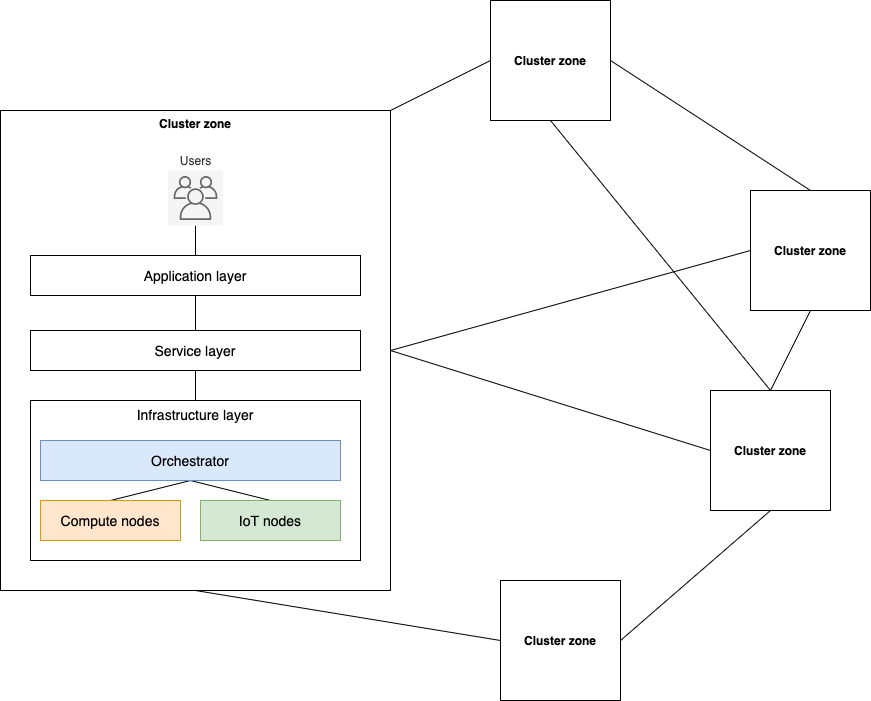
\includegraphics[width=0.75\columnwidth]{figures/architecture-federation}
\caption{A high-level view of a federated set of cluster nodes.} \label{fig:architecture-federation}
\end{figure}

Figure~\ref{fig:architecture-federation} depicts
the basic building blocks of the system, as we envision it to attain the sought dynamism of computation.  
\textit{Cluster nodes} allow forming flexible, agile, and geographically bound aggregates, called \textit{cluster zones}.
Each such zone federates the resources collectively available within its nodes, and orchestrates their deployment. 
%The rationale for a federation layer is two-fold.

The federation is achieved via a dedicated \textit{infrastructure layer}, which discovers and aggregates services, data and compute resources transparently across cluster nodes in a manner that meets end-to-end QoS requirements.

As we envision it, the system dynamically instantiates and schedules services along the path from source to destination, based on application-specific requirements and constraints. 
If a single cluster zone lacks hardware, software or data resources to meet the user needs, it will propagate the corresponding requests outside of its federation to cluster zones within an acceptable geographical distance that have the required capabilities.

Collaboration among cluster zones is essential to support user mobility across neighbouring regions. 
In the Continuum, services should follow the user movements without significant outage or perturbation.

User applications running on a single cluster node are given access to requested resources thanks to the intermediation of the \textit{service layer}. Applications intending to run on a cluster zone specify their service requirements and constraints, namely the type of resource (e.g., expected performance, pricing), without needing detailed knowledge of the underlying infrastructure. 
The \textit{orchestrator} receives the requirements from the \textit{service layer} intermediary and provisions resources and services as required, assigning them to \textit{compute nodes} in the target cluster zone.
While geographically distant, such nodes form an interconnected cluster that logically aggregates the available resources.

% \textcolor{red}{Applications are described as manifests, which itemise the relevant resources and service requirements.
% Resources concern for example the amount of CPU and memory.}
Services capture common dependencies like a database and persistent storage for data sources, along with pertinent constraints on them, such as latency limits and subscription plans.

We leave the federation architecture as an open research question for the future of the Continuum, owing to the comparatively early stage of maturation of our concept, and the broad and challenging scope of the topic. 
In the following, we limit ourselves to studying the infrastructure architecture, which is a fundamental enabler to the federation layer.

\subsection{Infrastructure architecture}

The infrastructure layer comprises a set of service providers that offer data and computational resources. The data can be generated by streaming IoT devices (e.g. cameras, smartwatches, and smart infrastructure). 
The computational resources can be heterogeneous and distributed through the infrastructure, from the Cloud to the Edge.

Figure~\ref{fig:architecture-broad} portrays the reference architecture of the Continuum infrastructure as we envision it. 
\begin{figure}[ht]
\centering
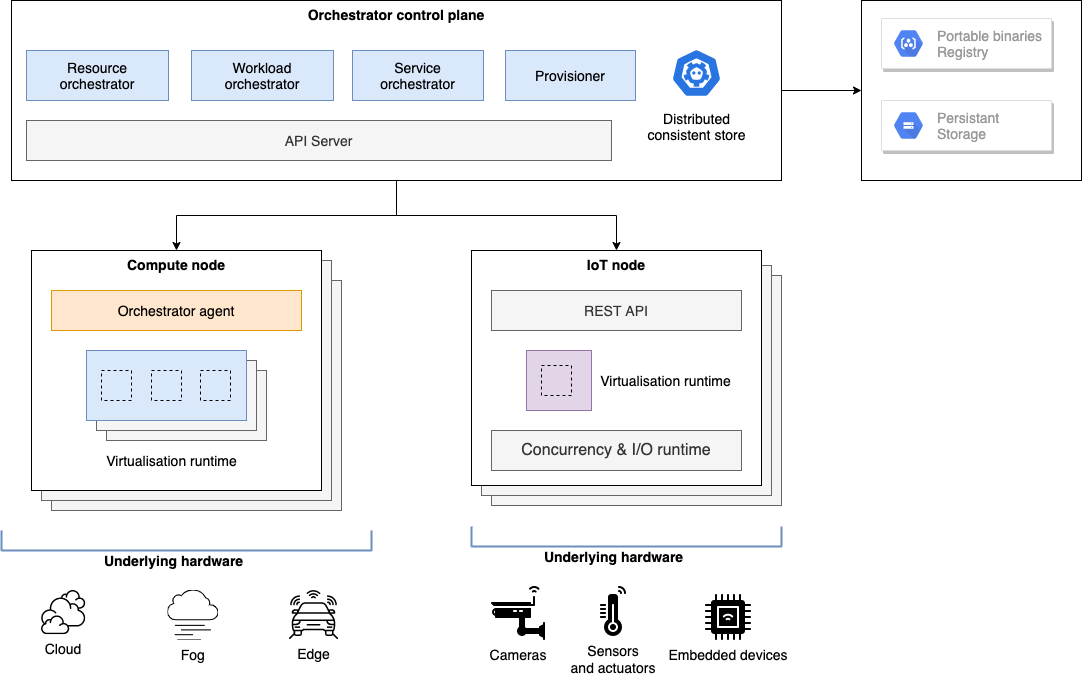
\includegraphics[width=\columnwidth]{figures/architecture-broad}
\caption{Reference architecture for the infrastructure.}
\label{fig:architecture-broad}
\end{figure}

\subsubsection{Orchestrator control plane}

The orchestrator control plane is the core of the orchestration system. It has a resource monitor module responsible for keeping track of real-time resource consumption metrics for each node in the compute cluster. The scheduler usually accesses this information to make better optimisation decisions. The scheduler is responsible for determining whether there are enough resources and services available in the Continuum to execute the submitted application. If resources are insufficient, applications can be rejected or put on wait until the resources are freed. Another possible solution is to increase the number of cluster nodes to host the incoming application. Such nodes can be provisioned from local machines or anywhere in the network, preferably close to the cluster. After determining if requirements can be satisfied, the scheduler maps application components onto the cluster resources. This deployment is done by considering the application requirements, e.g. latency, geographical constraints, availability or utilisation.

\subsubsection{Compute nodes}

Each machine in the cluster that is available for services and applications is a compute node. Each of these nodes implements the orchestrator agent runtime with various responsibilities. First, it collects local information such as resource consumption metrics periodically reported to the control plane. Second, it starts and stops service instances and manages local resources via a virtualisation runtime. Finally, it monitors the instances deployed on the node, sending periodic status reports to the control plane.

A critical requirement of the virtualization runtime on the Compute nodes is offering a consistent execution platform independent of any underlying infrastructure to allow applications to run across all software and hardware types with the same behaviour. This aspect is fundamental due to the extreme heterogeneity of the devices in the Continuum.

\subsubsection{IoT nodes}

IoT nodes are embedded devices that act as sensors or actuators, provided as services to the cluster (more on this to follow). The IoT nodes are heterogeneous in runtime implementation and communication protocols. Applications in the cluster interface with them via brokers provisioned by the cluster, as we discuss in Section §\ref{p:akri}. Besides, the embedded devices support dynamic configuration by running arbitrary virtualisation modules in a lightweight runtime.

Besides the requirement of interoperability between Compute nodes, the IoT runtime must as well be compatible with the application format accepted by the Compute nodes, assuming the module size and the hardware requirements can be satisfied by the limited device. Such extended service interoperability enables greater flexibility and novelty in deciding where some aspects of IoT computing, such as controlling and preprocessing, happens. 

Notably, solving how to run arbitrary computation on microcontrollers effectively allows opening the embedded world to the Continuum as an additional place of intelligent computing, rather than only as a mere data collector and dummy actuator.

\subsubsection{Underlying infrastructure}

One of the main requirements of the infrastructure architecture is the flexibility in being deployed on a multitude of platforms. Accordingly, the cluster machines can be either VMs on public or private Cloud infrastructures, physical machines on a cluster, or even mobile or Edge devices, among others. Such extreme diversity requires rethinking mainstream virtualization technologies in a form that doesn't require the application programmer to preemptively know the execution contexts.

\subsection{Use case: Weather-based services}\label{sec:uc}

As a practical example to guide the architecture's implementation, we apply the Continuum system design to weather-based services. The emergence of efficient sensing methods and IoT technologies are giving the opportunity to record and analyse possible influences of weather factors in both mainstream areas like flood warning~\cite{brzoza2016embedded} and novel fields like electrical load forecasting~\cite{weather-load-forecasting} and precision agriculture~\cite{keswani2019adapting}.

For instance, weather relevant attributes are of great significance for electrical load forecasting and include values like temperature, air pressure, vapour pressure, precipitation, evaporation, wind speed, and sunshine duration. An interesting addition is that detailed weather condition data sometimes may be captured solely by household sensors, such as the indoor temperature, sunshine duration, and indoor air quality, which differentiate in every house but have a strong effect on energy consumption. These data are also typically preprocessed to anonymise and normalise the final inputs. Gathering and preprocessing this data showcases how essential it is, for many services in the Continuum, that arbitrary code may execute safely and swiftly.

Additionally, typical parameters for precision agriculture are soil moisture content, soil temperature, surrounding temperature, humidity level, CO2 level of air, and sunlight intensity level. The sharing of weather parameters between electrical load forecasting and precision agriculture is, thus, an additional point in favour of sharing the data and computation on the Edge.

Finally, in a flood warning system, the telemetry stations acquire data (e.g. air humidity, soil moisture) from wireless sensors networks. Besides the opportunity of sharing this data with the above applications, the sensor networks also process the data in a distributed manner, and locally determine potential levee breaking. The geographical distance between the networks, the volume of data, and the relatively low interest (when no significant event is happening) make a centralised vertical solution undesired. In this case, the distributed architecture of the Continuum is a viable architecture for advanced telemetry services with distributed intelligence.

\begin{figure}[ht]
\centering
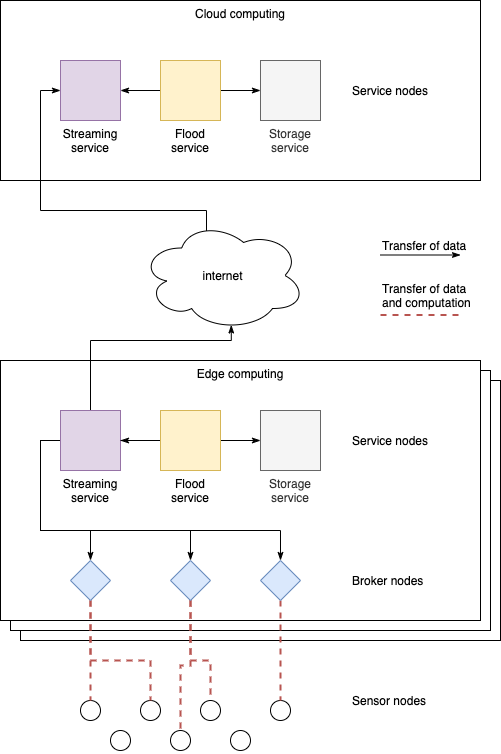
\includegraphics[width=0.7\textwidth]{figures/architecture-levee2}
\caption{Architecture for the flood warning system.}
\label{fig:architecture-levee}
\end{figure}

To meet the requirements of the cited types of services, we implemented a Proof of Concept system based on the architecture proposed in Figure~\ref{fig:architecture-levee}:

\begin{itemize}
    \item Sensor nodes: they are composed of sensor devices that collect data, preprocess it and transmit it to the Edge cluster for further processing. One challenging task of this layer is implementing the dynamic configuration of internal application-specific logic, as preprocessing is a necessary step presented in the case of electrical load forecasting;
    \item Broker nodes: they expose the sensor nodes behind a common interface. The broker subscribes to the IoT data and the device periodically sends updates, which are forwarded to the cluster. The broker ensures that both parts, IoT nodes and services nodes, are independent as far as they agree to communicate following the same API interface;
    \item Service nodes: they implement the needed services and allow them to be reused across different clusters. Internally each service can be composed of stand-alone services. We show the example of levee monitoring, which needs a streaming service to aggregate the data from the broker nodes, a local database to store the information for the analysis, and a flood prediction service to analyse the information and provide insight. 
\end{itemize}

The service nodes are deployed at multiple Edge clusters, corresponding to different stations, and at a Cloud cluster.

% The rationale for expanding the services to the Cloud is two-fold. First, the Edge clusters are heterogeneous in computing capacity, and some zones may have not enough computing power to handle streams. Leveraging the Cloud can help increase the workload at the cost of more bandwidth usage and latency. Such compromise might be acceptable, especially in the case of intensive data analysis on the sensor data.

The prediction model benefits from more knowledge derived from multiple streams geographically distributed. A flood risk assessment model running in the Cloud can achieve a globally optimal solution, whereas Edge services can output only locally optimal results. On the other hand, the communication channels may become unavailable during flood threat scenarios, so the system must perform a localised assessment. Unfortunately, the loss of communication is unpredictable, but the system must quickly adapt to that eventuality. All these examples of computing dynamism advocate that the Continuum shines compared to relatively static Cloud-only, Edge-only, or pre-defined Cloud+Edge architectures.

\section{The challenges ahead}
\label{sec:challenges}

Several challenges lay ahead in the realisation of the Continuum infrastructure. Besides featuring extreme heterogeneity, current Edge technology most notably lacks support for service orientation, interoperability, orchestration, reliability, efficiency, availability, and security. We now briefly discuss each problem in isolation and for each we later propose a candidate technology. Figure~\ref{fig:challenges-technologies} presents a preliminary overview.

\begin{table}
  \caption{Preliminary overview of the challenges and candidate technologies. WebAssembly is evidently a key enabling technologies in our research.}  \label{fig:challenges-technologies}
  \begin{tabular*}{\textwidth}{ | l | l }
   \toprule
    \textbf{Challenge} & \textbf{Technology} \\
   \midrule
    Service orientation & RESTful web services \\
    & Open Service Broker \\
    & CoAP \\
    \midrule
    Orchestration & Kubernetes, Akri \\
    Virtualisation & WebAssembly \\
    Dynamic configuration & WebAssembly \\
    Interoperability & WebAssembly \\
    Portability and Programmability & WebAssembly, Rust \\
   \bottomrule
  \end{tabular*}
\end{table}

\paragraph{Service orientation}\label{p:service-orientation}
We argue that service orientation is fundamental to organise and utilise distributed capabilities that may lie under the control of different ownership domains. 
% A Service-Oriented Architecture (SOA) provides "a uniform mean to offer, discover, interact with and use capabilities to produce desired effects consistent with measurable preconditions and expectations"~\cite{mackenzie2006reference}.

A service-oriented model is centred around a service provider that publishes its service interface (i.e., how users may access the corresponding functionalities) via a service registry where consumers may locate it and use it to bind to the desired service provider~\cite{haller2008internet}.

The prime virtue of such a model is the loose coupling it earns for services, which are solely responsible for the logic and information that they encapsulate, agnostic of the composition in which they can be aggregated by higher-level providers, and placed behind well-defined interfaces and service contracts with corresponding constraints and policies.
This design is in stark contrast with the dominant practice of the present day, where a multitude of ad-hoc programs are developed that are confined to single places of the network and permanently cement the behaviour of the associated devices~\cite{beckman2020harnessing}.

However, major limitations have to be overcome before services can be operated seamlessly and maintained nimbly.  

First and foremost, there is a lack of vendor-neutral, trustworthy and widely accepted service intermediaries. Their availability is critical to enable efficient retrieval of services that meet given user needs and warrant agreed levels of quality. Unfortunately, to date, interoperability is not dear to the main actors in the field \textcolor{red}{\cite{grozev2014inter}}.

A second critical limitation is the lack of inter-operable support for composing higher-order services from lower-level ones. 
Individual providers adopt their own conventions for interfaces and communication protocols: for example, Google Cloud Platform services heavily use Protocol Buffers~\cite{protobuf}, a Google technology for serialising structured data, in their service APIs. 
A plausible implementation of the Continuum should map high-level descriptions (e.g. key-value stores) to vendor-specific implementations.

Moreover, whereas services on the Internet of today are mute and unresponsive, future services should be communicative and reactive to their respective environments~\cite{haller2008internet}. 
The current service interfaces in fact are ostensibly designed with human interaction in mind, thus being scarcely suited for machine-to-machine (M2M) discovery and interaction. Effective M2M communication is paramout in our vision of the Continuum, as binding a consumer to a particular service interface should entail minimal direct interaction with the provider's infrastructure.

Finally, services fit for the Continuum, hence deployable at the Edge, are sensitive to the context of the environment in which they operate.
The context-awareness we envision is necessary to implement local control loops and trigger specific actions on local events (e.g. sensor readings in our PoC).

\paragraph{Orchestration}\label{p:orchestration}

The transition to the Continuum will require coordinating and scheduling the operation of multiple distributed service components. The complexity of that endeavour makes orchestration essential, over and above the rating it enjoys from DevOps adopters. 

Orchestrating in the Continuum is especially challenging owing to the scale, heterogeneity and diversity of resource types, and the uncertainties of the underlying environments for resource capacity (e.g. bandwidth and memory), network failures, user access pattern (e.g., for quantity and location), and service life cycle~\cite{BITTENCOURT2018134}.
Extreme heterogeneity also hinders devising sound pricing models that reflect account locations, resource types, transport volumes, and service latency.

Orchestrating services in the Continuum is a remarkable challenge, which encompasses technologies from various fields, including wireless cellular networks, distributed systems, virtualisation, platform management. Additionally, it requires mobility handover and service migration at local and global scales~\cite{Bittencourt201726}.

\paragraph{Virtualisation}\label{p:virtualisation}
\label{sec:virtualisation}

The rapid pace of innovation in data centres and application platforms has transformed how organisations build, deploy, and manage services.
Container-based virtualisation, owing to its natural versatility and light unitary weight, has become the dominant solution for all seekers of elastic scalability.
%\textcolor{red}{Born off Linux Containers (LXC)~\cite{bernstein2014containers}, modern containers are an OS-level virtualisation solution for running multiple isolated applications that all share a common underlying Linux kernel. 
%A container consists of one or more processes with reduced privileges and restricted visibility into kernel objects and host resources.}
Thousands of containers can be stored on a physical Cloud host in contrast with just very few traditional heavy-weight Virtual Machines. 
A natural near-future direction is an Edge-friendly containerisation that allows users to deploy services and applications on heterogeneous Edge nodes with minimal effort. 
Several works (e.g.~\cite{pahl2016container} and~\cite{bellavista2017feasibility}) argue the feasibility of container virtualisation applied to cheap low-powered devices, such as the Raspberry Pi. 

Thanks to the underlying Docker image technology~\cite{docker-image}, containers provide resource isolation, self-contained packaging, anywhere-deployment, and ease of orchestration, very fitting features for the Continuum.
% Several Cloud providers use this technology for their Platform-as-a-Service and Function-as-a-Service solutions. Modern serverless platforms (e.g., Google Cloud Functions, Azure Functions, AWS Lambda) isolate functional units in ephemeral, stateless containers. 
Nonetheless, we reckon that the current state of containerisation technology still comes at too great expense in terms of memory overhead and system requirements. A typical state-of-the-art Edge runtime for containers requires at least half a Gigabyte of memory even when idle~\cite{bohm2021profiling}. Besides, containers incur latency between hundreds of milliseconds and seconds, wholly unaffordable for latency-sensitive services that operate at the Edge. 
To achieve better efficiency, some platforms cache and reuse containers across multiple function calls within given time windows, typically 5~minutes. 
In the Edge, however, long-lived and over-provisioned containers can quickly exhaust local resource capacity, and become impractical for serving multiple IoT devices. 
% Supporting a large number of serverless functions while warranting low response time within tens of milliseconds~\cite{elbamby2019wireless}, thus is one of the main performance challenges for resource-constrained Edge nodes.

In the way of hard security, containers also offer weak isolation. To achieve stronger guarantees, they are often run in per-tenant VMs, too heavy for Edge or Fog nodes like the Raspberry Pi. 
A light\-weight yet robust isolation solution thus is a critical step in the quest for the Continuum.

\paragraph{Dynamic configuration}\label{p:dynamic-configuration}

IoT nodes must be capable of prompt reaction to context changes in the environment where they operate. Such reactions are critical to applications like video analysis~\cite{jang2018application} that are natural candidates for deployment at the extreme edge of the Continuum. 
% A risk scenario to be avoided is that IoT devices continue to operate needlessly or erroneously because their controllers running on nearby Edge nodes are late in making opportune adjustments.
Enabling dynamic configuration on constrained devices would enable swift adaptation to environmental events in accord with application requirements. 
This goal can be achieved by running an application-specific computation on the node itself, earning a considerable improvement in task accuracy (owing to physical vicinity), privacy preservation, network bandwidth, and response time.

Opening devices to arbitrary code execution, though, exposes the system to malicious acts, with compromising breaches that can exploit the slightest code weakness.
Current software isolation stacks like containers can hardly be used in trustworthy embedded systems as the latter typically lack the necessary storage capacity or Operating System components.

A further challenge of dynamic configuration is striking an acceptable compromise between warranting isolated execution and containing the corresponding loss of efficiency and increased energy consumption. A common memory-safe execution technique is to adopt interpreted languages that provide type and memory safety~\cite{jacobsson2020virtual, brzoza2016embedded}.

\paragraph{Interoperability}\label{p:interoperability}

Many technologies are available for connecting and integrating all kinds of "things" into the Continuum. 
ZigBee, IPv6 over Low-Power Wireless Area Networks (6LoWPAN), MQTT, and CoAP are popular in the wireless sensor networking area, while OPC has a good take-up in factory automation~\cite{al2020investigating}.
The fact is, though, that such technologies are too numerous and varied for any single standard to be able to accommodate all of them.

For this reason, building the Edge infrastructure of the Continuum requires coping with extreme heterogeneity, which standards will hardly be able to tame.
Best is to separate functionality from implementation, seeking interoperability in lieu of standardisation. Service-oriented architectures are ideal in this regard as they encapsulate functionality in services that can expose a common interface, abstracting away inner idiosyncrasies.

An infrastructure that allows connecting and integrating diverse technologies is not just a "necessary evil" but rather a strength that earns two key benefits. Firstly, it allows applying different solutions to different applications, in a best-fit logic. 
Secondly, an infrastructure where diverse technologies can easily be integrated into will be more future-resistant. 
Such flexibility is crucial for the Edge and IoT, which will undoubtedly see new developments for technologies and protocols. An infrastructure built with technology diversity in mind will allow interoperability with existing and already deployed devices and networks.
%\textcolor{red}{A similar level of heterogeneity occurs for Cloud platforms, which typically expose proprietary interfaces in isolated vertical solutions, which very much hamper cross-platform resource integration~\cite{grozev2014inter}. }

\paragraph{Portability and Programmability}\label{p:portability-and-programmability}
In Cloud-native models of computing, users of containerisation are free to select the programming language of choice, with the sole concern to ensure that the corresponding executable image, which embeds all the necessary package libraries and configurations, can be deployed on the target platform. 
Such images can be constructed from minimal file system layers, sharing read-only parts (e.g. base OS) with other containers, thus shedding a considerable footprint. 

Conversely, in the Continuum, the compute nodes are vastly diverse for CPU (e.g., x86\_64, ARM32, ARM64, and RISC-V) and runtime, making it much harder for programmers to make native application development and deployment decently portable. 

Docker images (and related tools like Docker buildx~\cite{docker-buildx}) attempt to overcome this challenge by defining multiple variants (usually referred to as tags) of the same image, to target multiple architectures, for processor or OS. 
However, this nice feature does not alleviate the pain of configuring and building each application image for all the target platforms and it is impractical to preemptively determine them in the Continuum.
% Besides, the lack of general-purpose OSs embeddable on Edge devices or their limitation in resource capacity impedes using conventional containers, further impairing portability across the Continuum.

% Portability also relates to programmability, in that the choice of programming language may favour or hinder portability. 

\section{Technology selection}\label{sec:technology-selection}

\subsection{Rationale for using open-source tools}

In order to address the described problems in our Proof of Concept (PoC), we adapted and integrated a variety of technologies from the industry. The resulting selection include a mixture of both well-known mainstream tools and experimental tools still under initial development.

The usage of existing tools is intentional to allow a realistic evaluation of the state-of-the-art to prove that there is an undeniable organic trend towards the Continuum. Besides, building over existing technologies will facilitate acceptance and ease the development.

\subsection{Service orientation}

The web has become the world's most successful vendor-independent application platform and the dominant architectural style on it is Representational State Transfer (REST)~\cite{rest} that makes information available as resources identified by URIs. The web is a loosely coupled architecture and applications communicate by exchanging representations of these resources using the HTTP protocol. HTTP is the most popular application protocol on the Internet and the pillar of the Web. However, new communication protocols (e.g. CoAP, which we discuss in Section \ref{sec:coap}) are emerging to extend the web to the Internet of Things and HTTP itself is undergoing revisions (e.g. HTTP/3 or QUIC~\cite{langley2017quic}).

Our rationale for picking REST is threefold.\par
First, REST resources are an information abstraction that allows servers to make any information or service available, identified via Uniform Resource Identifiers (URIs). For example, this allows the sensor nodes in our PoC to act as a server and own the resource's original state. The client negotiates and accesses a representation of it. Such representation negotiation is suitable for interoperability, caching, proxying, and redirecting requests and responses. These features enable seamless inter-operation and better availability of any kind of service in the Continuum, especially IoT-involved services. Besides, under the REST architectural paradigm, IoT nodes can advertise web links to other resources creating a distributed discoverable IoT web and resulting in an even more scalable and flexible architecture.\par
Second, REST allows to use a uniform interface across the Continuum: clients access the server-controlled resources in a request-response fashion using a small set of methods with different semantics (GET, PUT, POST, DELETE). The requests are directed to resources using a generic interface with standard semantics that intermediaries can interpret. The result is an application that allows for layers of transformation and indirection independent of the information origin. \par
Third and last, REST enables high-level interoperability between RESTful protocols through proxies or, more generally, intermediaries that behave as server to a client and play as client with respect to another server. REST intermediaries fit well with the assumption that not every device must offer RESTful interfaces directly. Such flexibility suitably accommodates the diversity of communication protocols on the Edge.

We used these features to bring IoT nodes into the Continuum as any other service and to enable the coexistence of multiple equivalent services offered by different Cloud providers. We mapped provider-specific interfaces to uniform RESTful interfaces.

% In several cases, notably in the Internet of Things, it may not be possible to change the underlying communication protocol. However, intermediaries allow exposing the resources through a RESTful API nevertheless. The interactions behind that RESTful interface are invisible and may include highly specialised protocols for the specific implementation scenario (e.g. OPC UA or MQTT)~\cite{guinard2010resource};
    % \item Communication protocol independence: Public APIs benefit from the adoption of HTTP because it leads to an API accessible from all programming languages and environments without additional technology. On the other hand, HTTP is relatively expensive for both binary overhead and network resource usage. Fortunately, the REST architectural style is not strictly tied to HTTP, and new communication protocols like CoAP (§\ref{sec:coap}) can offer a very similar interface while guaranteeing more lightweight implementation, less demand for network bandwidth, lower latency and more energy efficiency among many features;
    % \item Machine-to-Machine communication (M2M): communication protocols must be specifically designed for efficient M2M communications without introducing overhead in network load, delay, and data processing. In the M2M environments typical of IoT applications (and of the Continuum, by extension), devices must discover each other and their resources. New approaches from the IETF include the well-known resource path \emph{/.well-known/scheme} (RFC 5785) and the HTTP link header (RFC 5988);
    % \item \textcolor{red}{Stateless: REST requires requests from clients to be self-contained, in the sense that all information to serve the request must be part of the request. Statelessness helps applications to scale, as persisting state in a highly distributed system brings challenges like consistency and hinders support for user mobility in the Continuum space.}

% \textcolor{red}{From the previous points, it is clear that the design goals of RESTful web systems and the benefits for a decentralised and massive-scale service system align well with the field of pervasive computing. For these reasons, REST an ideal candidate to build a universal API for services and devices in the Continuum, letting developers reuse their existing skills and tools. }

\paragraph{Open Service Broker}

\begin{figure}[ht]
\centering
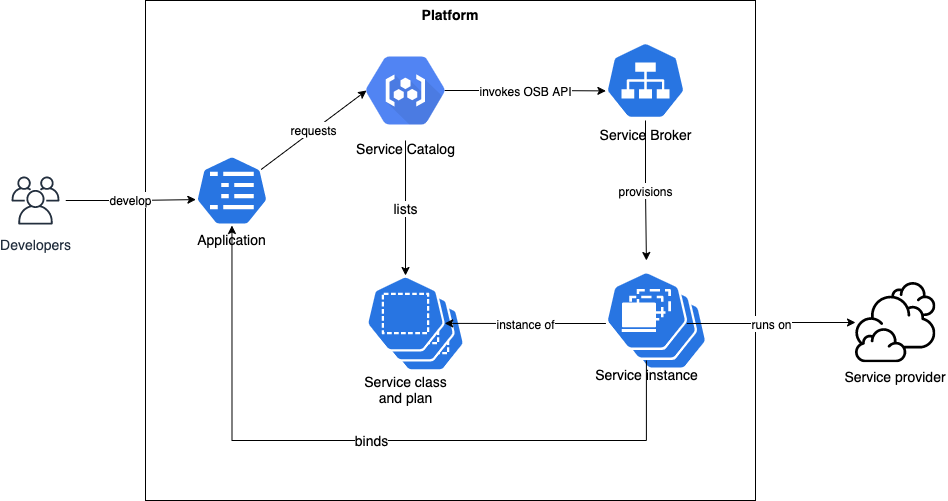
\includegraphics[width=\columnwidth]{figures/osb}
\caption{The Open Service Broker architecture.} \label{fig:osb}
\end{figure}

In our PoC, we realised a web-based service platform that implements the RESTful Open Service Broker (OSB) interface~\cite{osb}. Components that implement the OSB REST endpoints are referred to as service brokers and can be hosted anywhere the application platform can reach them. Service brokers offer a catalogue of services, payment plans and user-facing metadata. The main components of the OSB architecture are depicted in Figure~\ref{fig:osb}.

In the Continuum platform, providers control access to services and payment plans but permit developers to add their own services to the catalogue. In this manner, we expect that over time a rich ecosystem of services may be developed and tapped from simple well-documented RESTful interfaces.

As Cloud standards still struggle to gain traction, however, we need to bridge the heterogeneity gap between platforms. 
To this end, we used brokers to orchestrate resources at different levels within a provider. As the number of Cloud vendors is limited, building brokering layers that align access to different Clouds is an affordable endeavor. The service broker translates RESTful requests from the platform to service-specific operations such as creating, updating, deleting, and generating credentials to access the provisioned services from applications. Service brokers can offer as many services and plans as desired. Multiple service brokers can be registered with the service platform so that the final catalogue of services is the aggregate of all services. The platform is thus able to provide a rich catalogue and a consistent experience for application developers who consume these services.

Over the years, the API interface of the OSB has matured considerably, learning from the experience of a wide range of marketplace services and Cloud vendors, such as Microsoft Azure and Huawei Cloud. The current standard version 2.17 is entirely designed around asynchronously provisioned services and provides valuable guidance for challenging situations such as service failures. 
The OSB guidance ensures consistent semantics and interoperability across various service behaviours.
Sadly though, service dependency remains a pain point that needs to be coped with, as for example in the architecture we devised for our use case (Figure \ref{fig:architecture-levee}). 
Currently, the OSB standard does not support a parent-child relationship model between services, whose handling is left inconveniently to the discretion of the broker author. 
The problems that arise from service dependency include whether to publish multiple services as standalone packages and how to share credentials between services, provision and remove them in the proper order, and solve all these issues uniformly across all platforms.

\paragraph{CoAP}\label{sec:coap}

\begin{figure}[ht]
\centering
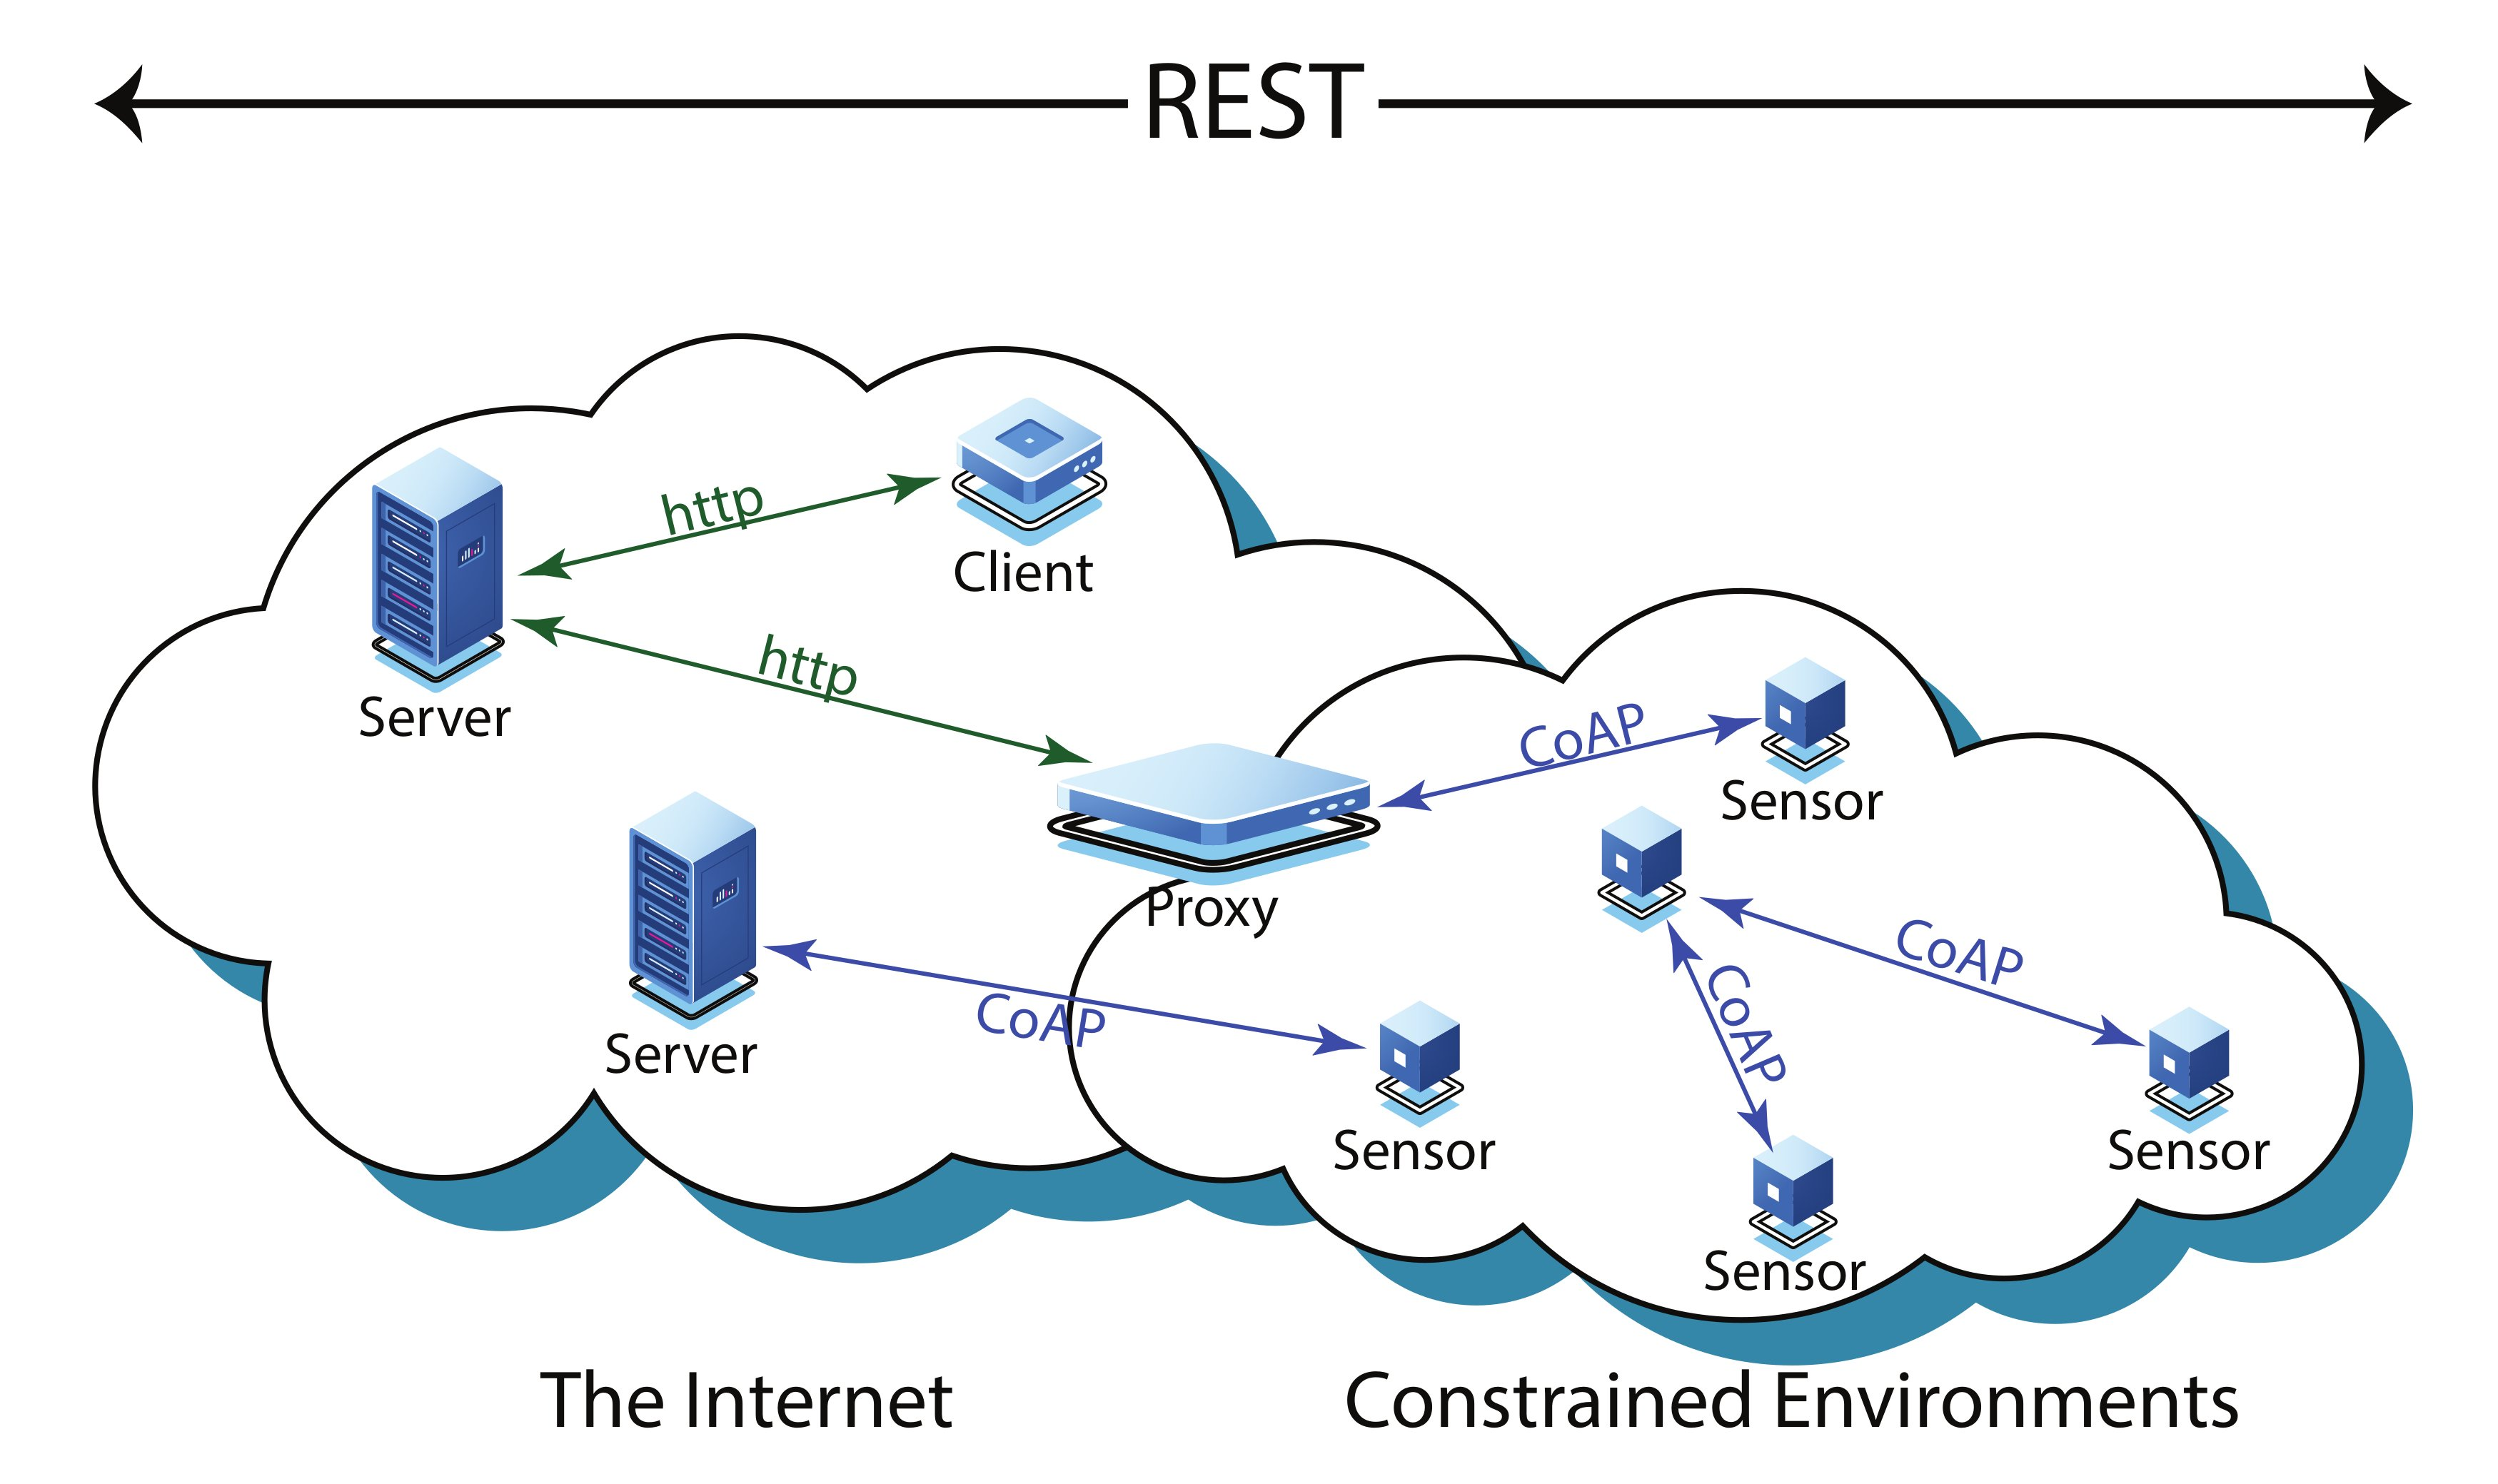
\includegraphics[width=\columnwidth]{figures/coap}
\caption{The REST architecture enhanced with CoAP. Source~\cite{bormann2012coap}.}
\label{fig:coap}
\end{figure}

To include IoT nodes in our REST architecture, we adopted CoAP~\cite{bormann2012coap}, a web communication protocol for use with constrained nodes and constrained (e.g. low-power, lossy) networks. A central element of CoAP's reduced complexity compared to HTTP is that it uses the UDP transport protocol instead of TCP and defines a very simple message layer for retransmitting lost packets.

The protocol is designed for M2M applications and provides a RESTful architecture between IoT nodes, supporting built-in discovery of resources. As a result, CoAP easily interfaces with HTTP for integration with web services while meeting specialised IoT requirements such as multicast support, very low overhead and simplicity for constrained environments. 

% The rationale for UDP is that TCP carries significant overhead and can have suboptimal performance for links with high packet loss, both of which are common across the Internet~\cite{nygren2010akamai} and especially on remote locations where sensors might be deployed. Besides, the HTTP protocol adds further burden, as the additionally multiple round trips required for the requests can quickly add up, affecting the device performance and energy efficiency.

% CoAP uses a four-byte binary header within UDP packets, followed by a sequence of options, each up to two bytes. The protocol's specification also defines the usual four request methods: GET, PUT, POST, and DELETE. Similarly, response codes are patterned after the HTTP response codes.

% The URI format allows exposing device data as resources and the use of standard and specialised service endpoints. For instance, CoAP servers are encouraged to provide resource descriptions via the well-known URI \emph{/.well-known/core} to achieve resource discovery. Clients then access this description with a GET request on that URI, usually via an IPv4 or IPv6 broadcast message. The description format is based on the CoRE Link Format (RFC 6690), which is simple and easy to parse. Ease of parsing allows more efficient M2M discovery and inter-communication between the nodes themselves.

% The CoAP protocol supports different resource representations, in line with the REST architecture's representation negotiation. The default format is textual for its convenience when reading and parsing. The binary format is efficient to communicate but requires external tools to make it readable by human users. XML is understandable and very well structured, but the size of its messages is significant, and it is much worse to parse than binary formats. Lastly, JSON is understandable, well structured and compact, but may still put an unnecessary parsing burden on the limited device. With all constrained devices, flash or memory consumption is one of the biggest problems, notably on devices where network connectivity already claims significant buffer memory.

% Another advantage of CoAP is that it supports a familiar and intuitive pattern already in use for development with standard web technologies, which affords a smoother learning curve. 
%This feature cannot be underestimated as allowing developers to use a familiar and seamless programming experience is essential to achieve Continuum's success.

We made CoAP nodes interoperable with the rest of the Continuum by following the REST architecture's proxy pattern, as depicted in Figure~\ref{fig:coap}. We built intermediaries (discussed in §\ref{p:akri}) that speak CoAP on one side and HTTP on the other without encoding specific application knowledge. Because equivalent methods, response codes, and options are present in HTTP and CoAP protocols, the mapping between them is straightforward. Consequently, the intermediary can discover CoAP resources and make them available at regular HTTP URIs, enabling web services in the Continuum to access CoAP servers transparently in the OSB service platform.

% \textcolor{red}{However, the HTTP client-initiated interaction model may be unsuited for many event-based and streaming systems in the IoT. Data is sent asynchronously to the clients as soon as it is produced. CoAP uses the Observe approach (RFC 7641) to support pushing information from servers to clients to overcome this issue. A client can indicate its interest in further updates from a resource by specifying the "Observe" option in a GET request. If the server accepts this option, the client becomes an observer of this resource and receives an asynchronous notification message each time it changes. This kind of communication, combined with an intermediary broker, allows streaming data updates via WebSocket (RFC 6455) and overcoming the client-pull interaction model of HTTP. The broker can also help achieve more reliable communication by transparently changing the underlying sensor in case of unavailability or by avoiding closing the connection in case of temporary loss of connectivity.}

\subsection{Orchestration}

Kubernetes~\cite{kubernetes} is an open-source orchestration framework designed to manage containerised workloads on clusters, originated from Google's experience with Cloud services. Two notable features make Kubernetes especially attractive for our PoC. 
First, thanks to the Container Runtime Interface (CRI) API standardisation, Kubernetes allows for various container runtimes from a technical perspective, with Docker natively supported by the platform. This extensibility allowed us to leverage a uniform virtualisation platform based on WebAssembly, while leaving the single Compute and IoT node to decide the most appropriate runtime (e.g. an interpreter compared to Just-in-Time or Ahead-of-Time compiler).

Second, Kubernetes provides users with a wide range of options for managing their Pods (the most basic unit of deployment in Kubernetes) and how they are scheduled, even allowing for pluggable customised schedulers to be easily integrated into the system. Notably, it also supports label-based constraints for the Pods' deployment. Developers can define their labels to specify identifying attributes of objects that are meaningful and relevant to them but that do not reflect the characteristics or semantics of the system directly. 
%An example would allow specifying that an IoT device component must be reachable from the host. 
More importantly, labels can be used also to force the scheduler to colocate services that communicate predominantly within the same availability zone, which improves latency very much and paves the way for context-aware services. % However, to realise the heterogeneity goals, it is required to filter unqualified resources continuously. New resource affinity models should be proposed to rank the resources when provisioning for different applications.

% The basic building block in Kubernetes is a Pod. A Pod encapsulates one or more tightly coupled containers that are colocated and share the same set of resources. Pods also encapsulate storage resources, a network IP, and a set of options that govern how the Pod's container(s) should run. A Pod is designed to run a single instance of an application enabling horizontal scaling by replicating multiple Pods across the nodes. The amount of CPU, memory, and ephemeral storage a container needs can be specified when creating a Pod. This information can then be used to make decisions on Pod placement. These compute resources can be specified as both requests and limits.

% Moreover, etcd~\cite{etcd} is an open-source highly available distributed key-value store and a fundamental part in supporting Kubernetes in managing the cluster nodes and jobs. Specifically, etcd is used to store all of the cluster's data and acts as the single source of truth for all of the framework's components.

% \textcolor{red}{Overall, Kubernetes is a highly mature system; it stemmed from 10 years of experience at Google. It is the leading container-based cluster management system with an extensive community-driven support and development base. It provides users with a wide range of options for managing their Pods and how they are scheduled, even allowing for pluggable customised schedulers to be easily integrated into the system.}

One more reason for our picking Kubernetes over Docker Swarm~\cite{docker-swarm} was lack of multitenancy in the latter. 
Docker Swarm is a popular open-source orchestrator often cited for Edge orchestration (e.g.~\cite{bellavista2017feasibility}, and~\cite{ismail2015evaluation}) due to its simplicity. However, support for multitenancy is a must for our service platform.

\paragraph{Akri}\label{p:akri}

\begin{figure}[ht]
\centering
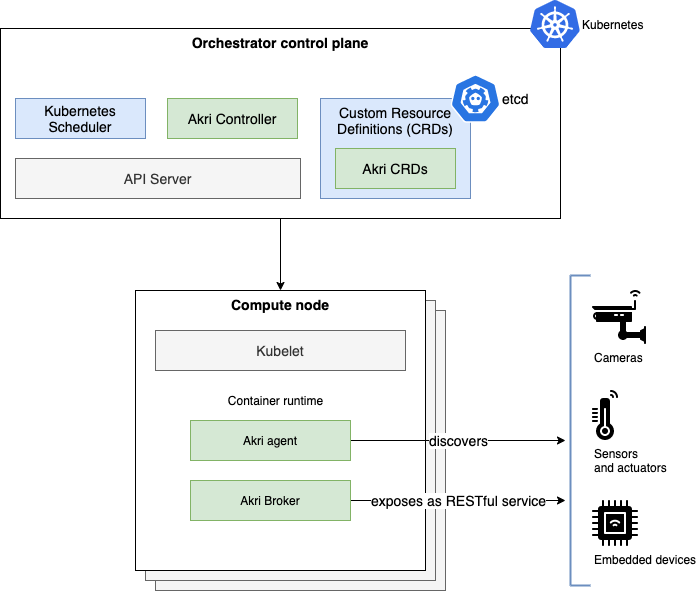
\includegraphics[width=\columnwidth]{figures/akri}
\caption{The Akri architecture can be divided into four main components: the agents, the controller, the brokers and the configuration. A configuration extends the Kubernetes API with new communication protocols and the related metadata, such as the protocol discovery parameters or the Docker image for the agent container. The Akri agent is a Pod responsible for discovering devices according to a communication protocol. It keeps track the device's state and communicates status updates with the Akri controller.}
\label{fig:akri}
\end{figure}

To register the IoT devices on the Kubernetes cluster, we adopted Akri~\cite{akri}, a preliminary Microsoft open-source project which allows visibility to IoT devices from applications running within the Kubernetes cluster. Akri stretches Kubernetes' already experimental APIs to implement the discovery of IoT devices, with support for the diversity of communication protocols and ephemeral availability.

% At the time of writing, the project has built-in support for ONVIF~\cite{onvif}, udev~\cite{udev} and OCP UA~\cite{gruner2016restful} discovery handlers, with an incoming proposal for CoAP~\cite{bormann2012coap} by us.

Using Akri, the Kubernetes cluster can carry out dynamic discovery to use new resources as they become available and move away from decommissioned/failed resources. Discovering IoT devices is usually accomplished by scanning all connected communication interfaces and enlisting all locally available resources.

Akri is also responsible for enabling applications to communicate with the device and deploying a broker Pod as intermediary. We devised the broker as a web server that abstracts the actual communication between devices and applications behind the RESTful API described Previously.

% Akri should automatically find all the devices in the environment and make them available as web resources. For instance, the agent regularly discovers the devices by scanning for CoAP resources.

% The broker may also offer local aggregates of device-level services, such as the combined temperature measurements of all the Things connected to it for later consumption in our flood prediction, electrical load forecasting services or precision agriculture services.

Our RESTful broker also helps to scale the number of concurrent HTTP requests by implementing highly performant cache mechanisms. The IoT resource periodically sends its sensor readings to the broker, where the values are cached locally. Each application request is then served directly from this cache without accessing the actual device, with benefits on the average roundtrip time.

% The broker architecture has the advantage of fully decoupling the leaf node from the cluster workload. It only needs to send an update packet with a frequency short enough to ensure data validity. On the other hand, the retrieved data's staleness will depend on the device's frequency of updates. Forwarding the HTTP request (adequately translated) has the advantage of always returning the most recent sensor reading when the request is processed. The cache mechanism cannot be applied for non-cacheable requests (e.g. HTTP POST) that must be sent to devices, such as turning on LEDs or changing the application state.

As many distributed monitoring applications are usually read-only during their operation (e.g. sensors collecting data in our case), this architecture exhibits great scalability. A potential goal is to enable new types of services where physical sensors can be shared with thousands of users with little impact on latency and data staleness. However, at the time of writing, this is still a very distant achievement.

The Kubernetes Device Plugin API heavily influences the current Akri architecture. Such interface, already considered experimental by the Kubernetes community, was designed for hardware attached to compute nodes, e.g. GPUs. However, IoT devices can live independently from the nodes, and most of them do. Akri expects a 1:1 relationship between compute node and device, whereas most IoT devices do not have any kind of relationship to any node per se. This mismatch has several undesired consequences, including, principally, scalability and resiliency.

Another pain point in Akri's current state is that the project lacks more advanced yet very needed features for implementing software caching or assuring high availability or autoscaling in IoT scenarios. Such features are admittedly harder to provide but highly needed to bring the Cloud to the Edge and vice versa, an essential preliminary step to the Continuum.

\subsection{Virtualisation, Interoperability and Portability}\label{sec:virtualization}

% \begin{figure}[ht]
% \centering
% 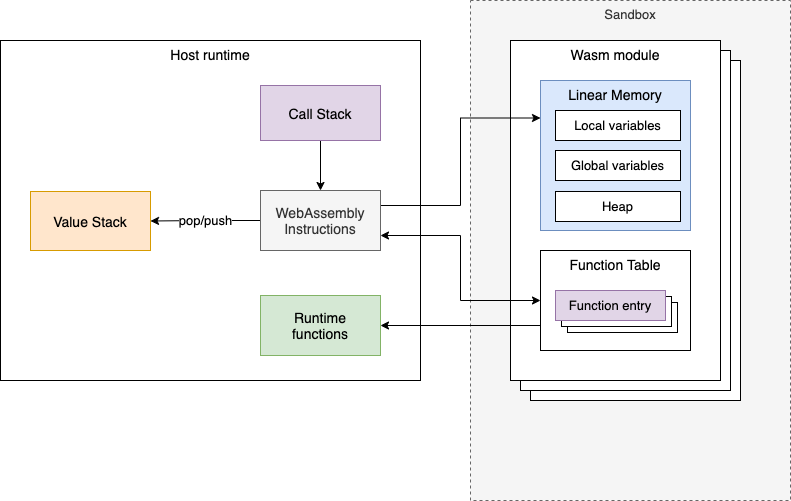
\includegraphics[width=\columnwidth]{figures/webassembly}
% \caption{WebAssembly stack machine.} \label{fig:webassembly}
% \end{figure}

WebAssembly (Wasm)~\cite{haas2017bringing}, first announced in 2015 and released as a Minimum Viable Product in 2017, is a nascent technology that provides strong memory isolation (through sandboxing) at near-native performance with a much smaller memory footprint. WebAssembly is a language designed to address safe, fast, portable low-level code on the web. Developers who wish to leverage WebAssembly may write their code in a higher-level (compared to bytecode) language such as C++ or Rust~\cite{aws-rust} and compile it into a portable binary that runs on a stack-based virtual machine.

% \textcolor{red}{Even though WebAssembly technically is a binary code format, it can be presented as a language with syntax and structure. This design choice was intentional since it makes it easier to explain and understand without compromising compactness or decoding ease.}

% A Wasm binary takes the form of one or more modules. It contains definitions for functions, globals, tables, and memories. 

% The computation is based on a stack machine represented in Figure~\ref{fig:webassembly}: code for a function consists of instructions that manipulate values on an implicit operand stack, popping argument values and pushing result values. However, WebAssembly represents control flow differently from most stack machines. It does not offer simple jumps but instead provides Structured Control Flow (SCF) constructs more akin to a programming language. This design ensures by construction that control flow cannot contain arbitrary branches. The SCF allows WebAssembly code to be validated and compiled in a single pass as well. SCF can also be disassembled to a WebAssembly text format (.wat) that is easier to read and often overlooked but crucial human factor on the web.

% A WebAssembly program's memory is a large array of bytes referred to as a linear memory or simply memory. All memory access is dynamically checked against the memory size, and out of bounds access results in a trap. Linear memory is disjoint from code space, the execution stack, and the engine's data structures. 

% \textcolor{red}{Each Wasm memory access addresses linear memory at an offset from the base, $n$, of the linear memory. Thus, some address virtualisation as an address $b$ in the sandbox is located at $b + n$ in physical memory.} The Wasm runtime is responsible for translating linear memory accesses and bounds-checking them to prevent accesses outside the sandbox.

% \textcolor{red}{Additionally, it allows a WebAssembly engine to be embedded into any other language runtime without violating memory safety and enabling programs with many independent instances to exist in the same process.} These sandboxing features make WebAssembly a compelling technology upon which to implement a virtualisation stack for the Continuum. On the Continuum web, code is fetched from untrusted sources, and it is vital that it can be safely executed on a plethora of language runtimes.

% Another critical safety feature of Wasm is the type system. Code must be validated before it can be executed safely. Validation rules for WebAssembly are defined succinctly as a type system. This type system is, by design, simple. It is designed to be efficiently checkable in a single linear pass to allow parallelisable binary decoding and compilation.
% Moreover, function pointers cannot be dereferenced directly. A call to a function pointer is translated into a function in a runtime table of valid entry points and types. The type of the function is checked dynamically against the expected type in the said entry. The dynamic signature check protects the integrity of the execution environment. In case of a type mismatch or an out of bounds table access, a trap occurs.

We picked WebAssembly as the technology enabling virtualisation, interoperability and portability in the Continuum for two fundamental reasons. 
First, WebAssembly provides language, hardware, and platform independency by offering a \textit{consistent} execution platform independent of any underlying infrastructure to allow applications to run across all software and hardware types with the same behaviour. The importance of such a feature for the Continuum cannot be emphasised enough.
Second, WebAssembly is advertised as safe \textit{and} fast to execute. A program code cannot corrupt their execution environment, jump to arbitrary locations, or perform other undefined behaviour (which memory-safe languages such as Rust, contribute to preventing). Thanks to that execution guarantee, a WebAssembly may suffer only data exploits, which are mitigated by applying memory and state encapsulation at the module level rather than the application level.
% In that manner, a module's memory and functions cannot leak information unless explicitly exported/returned. 
% This granularity in sandboxing is extremely important as security incidents have increasingly exploited vulnerabilities in the dependency chain. Reuse of third-party software is pervasive in modern languages like JavaScript, Rust or Go. 
Granular memory encapsulation means that even untrusted modules can be safely executed in the same address space as other code, a critical point for dynamic configuration in constrained devices and multitenancy in the Compute nodes of our architecture. Performance wise, benchmarks of Wasm runtimes on modern browsers have shown a slowdown of approximately 10\% compared to native execution, typically within 2x~\cite{haas2017bringing, menetrey2022webassembly}.
% Third, the Wasm binary code is designed to be compact, streamable and parallelisable. Code transmitted over the network has to be as compact as possible to reduce load times in compute nodes, save potentially expensive bandwidth and reduce memory usage on constrained network-attached devices. For example, a Wasm runtime can minimise latency by starting and parallelising streaming compilation as soon as function bodies arrive over the network, differently from container images. Reducing latency is essential for increased mobility, quick release of resources, and support for low-latency use cases.

    % \item \emph{Deterministic and easy to reason about}: WebAssembly has been designed with formal semantics from the start for both execution and validation. Besides, the Wasm binary can be compiled into a .wat file to simplify learning and debugging;
    % \item \emph{Simple interoperability}: WebAssembly is similar to a virtual ISA in that it does not define how programs are loaded into the execution engine or how they perform I/O. The embedder (i.e. the host runtime) defines how modules are loaded, how imports and exports between modules are resolved, provides foreign functions to accomplish I/O, and specifies how traps are handled. It is possible, by design, to link multiple modules that different authors have created from likewise different source languages. However, as a low-level language, WebAssembly does not provide any built-in object model. It is up to developers to map their data types to numbers or memory. This design is supposed to provide maximum flexibility to developers, and unlike previous VMs like Java or .NET, it does not privilege any specific programming or object model while penalising others. The downside of this design is that interoperability with object references is cumbersome. It involves exchanging references between the Wasm application and the host code or between modules that originated from different languages. A step in easing this issue is the recent introduction of Reference Types~\cite{reference-types}. On the other hand, since WebAssembly is a virtual ISA, not over a programming language, a WebAssembly module may be compiled once and moved freely between different hardware architectures with no recompilation;
    % \item \emph{Easy to validate and compile}: validation proceeds by checking on the fly while the incoming bytecodes arrive, with no intermediate representation (IR) being constructed. Benchmarks run on mainstream browsers in~\cite{haas2017bringing} prove that validation can be fast enough to be performed at a full network speed of 1Gib/s;

% Despite the name WebAssembly, there has been a significant effort in the last years in adopting Wasm for native execution, as it is a portable target for the compilation of various high-level languages. Wasm standard does not necessarily make browser-specific assumptions, and there has been substantial work to standardise the WebAssembly System Interface (WASI) to run Wasm outside the browser.

% To the best of the authors' knowledge, the original design goals assumed a browser-based execution context. Nevertheless, such goals fit perfectly the Continuum's needs, where the web is the infrastructure upon which applications and services are deployed. On this matter, browsers are very much akin to an Operative System for client web applications, and WebAssembly is thus unsurprisingly being adopted on conventional OSes as well. Native execution and browser execution share many problems, like isolation, portability and interoperability, to name just a few.

% At the time of writing, there are several Wasm runtimes for programs written in different languages capable of embedding Wasm applications. On the other hand, multiple compilers can compile languages to Wasm.

% as shown in Figure~\ref{fig:portability}. Notably, the Wasm backend for LLVM~\cite{llvm} works for C, C++, and Rust. Commercial solutions have also been slowly but steadily gaining popularity. Cloudflare's Service Workers~\cite{Cloudflare-workers} began to offer support for creating and hosting serverless functions in WebAssembly. In March 2019, the edge-computing platform Fastly had announced an open-sourced Lucet~\cite{fastly-lucet} that provides a compiler and runtime to enable native execution of Wasm applications and can instantiate a Wasm module within $50\mu s$, with just a few kilobytes of memory overhead. Parity is also actively experimenting with writing smart contracts using Wasm~\cite{parity-wasm}.

WebAssembly is currently looked at as a candidate method for running portable applications without containers. Ideally, WebAssembly can provide significantly more lightweight isolation than VMs and containers for multi-tenant service execution. This idea is still in its infancy, but there has been some interest in recent years (\cite{hall2019execution},~\cite{gadepalli2020sledge} and~\cite{shillaker2020faasm}), especially for serverless computing.

\subsubsection{Dynamic configuration}

Another strong point of WebAssembly is enabling arbitrary code execution on highly constrained devices on the Continuum. The authors of~\cite{10.1007/978-3-030-29897-5_33} and~\cite{peach2020ewasm} have also explored various WebAssembly-based mechanisms for safe arbitrary execution on constrained devices and have evaluated the trade-offs between efficient Wasm processing and memory consumption. Generally speaking, Just-In-Time compilers for WebAssembly exist (e.g. Wasmtime~\cite{wasmtime}) and receive more attention from the community, but their size and complexity make them unsuitable as yet for microcontrollers.

Although WebAssembly interpreters can often be approximately 11x slower than native C~\cite{wasm3-performance}, they help dynamically update system code and debugging but are not yet mature in terms of performance and energy efficiency.

Interpreting WebAssembly on microcontrollers offers an appealing alternative to other language runtimes. The WebAssembly standard has many features that make it attractive for embedded devices~\cite{peach2020ewasm}. First, as mentioned before, WebAssembly can be generated from different source languages and run on many CPU architectures. Furthermore, many broadly used language runtimes such as JavaScript, Lua, or Python cannot provide predictable execution. They may require excessive memory for a microcontroller, whereas Wasm requires no mandatory garbage collection and only a few runtime features around maintaining memory sandboxing. This lightweight-ness is a most valuable asset in an embedded adaptation. \\

% \subsection{Programmability}
% \label{p:Rust}

% As the Continuum integrates compute support across the network, the attack surface dramatically increases with it. Notably, the leading cause of security vulnerabilities are memory safety bugs like data races and buffer overflows. Security has to be a top priority during software development, yet most infrastructure is programmed with C and C++. These two programming languages are chosen due to the low memory footprint and the high processing performance endowed by their very nimble runtime. Embedded systems have favoured the two languages because of the need for low-level control over the hardware. However, C and C++ do not excel at producing secure software, as evidenced by the many vulnerabilities reported against the software written in them~\cite{cwe}.

% Conversely, Rust is a strongly-typed, compiled language that uses a lightweight runtime similar to C. Unlike many other modern languages, Rust is an attractive choice for predictable performance because it does not use a garbage collector. It provides strong memory safety guarantees by focusing on "zero-cost abstractions", meaning that safety checks are done at compile-time and runtime checks (e.g. out-of-bounds access) have the minimum overhead and come with a predictable cost.

% Safe Rust code is guaranteed to be free of null or dangling pointer dereferences, invalid variable values (e.g. casts are checked), reads from uninitialised memory, unsafe mutations of shared data, and data races, among other misbehaviours. The borrow checker, the most innovative feature of the language compiler, runs as part of the compilation process and catches bugs like just mentioned misbehaviours. 

% Lastly, thanks to integration with LLVM, the Rust compiler can transform the Intermediate Representation (IR) of the program to generate WebAssembly binary code. The union of Rust and WebAssembly constitutes a powerful combination. Developers can write source code in Rust to achieve high productivity and efficient memory-safe applications. WebAssembly can contribute with a hardened execution environment and universally portable binaries. Developers do not need to compile or distribute multiple versions (e.g. Docker image versions) of the same software.

% Besides being a system language, we found Rust a sensible choice to build \emph{any} reliable and performant software. We used it successfully throughout our work in the Continuum. We were able to run a WebAssembly interpreter and CoAP server on top of a minimal embedded runtime for highly constrained environments like microcontrollers. Later we leveraged the same language and developer experience while working on systems-level programming in Krustlet and cluster-level communication with Akri in Kubernetes. Lastly, we also implemented the protocol-bridging brokers and high-level web services in Rust. Despite the diversity of programming levels, the fast-paced Rust community is extremely rich in libraries for a variety of use cases. Admittedly, though, a good level of craftsmanship is still required as most open-source libraries are not battle-tested and present rough edges, like unimplemented yet critical features, which one has to develop independently. Additionally, embedded or low-level system programming may require using unstable language features, which hinders the adoption of Rust for critical, long-lived applications or even industry-wide adoption in production.\\

Figure~\ref{fig:architecture-technologies} summarises the key technologies we employed in the reference architecture of the Continuum infrastructure.

\begin{figure}[ht]
\centering
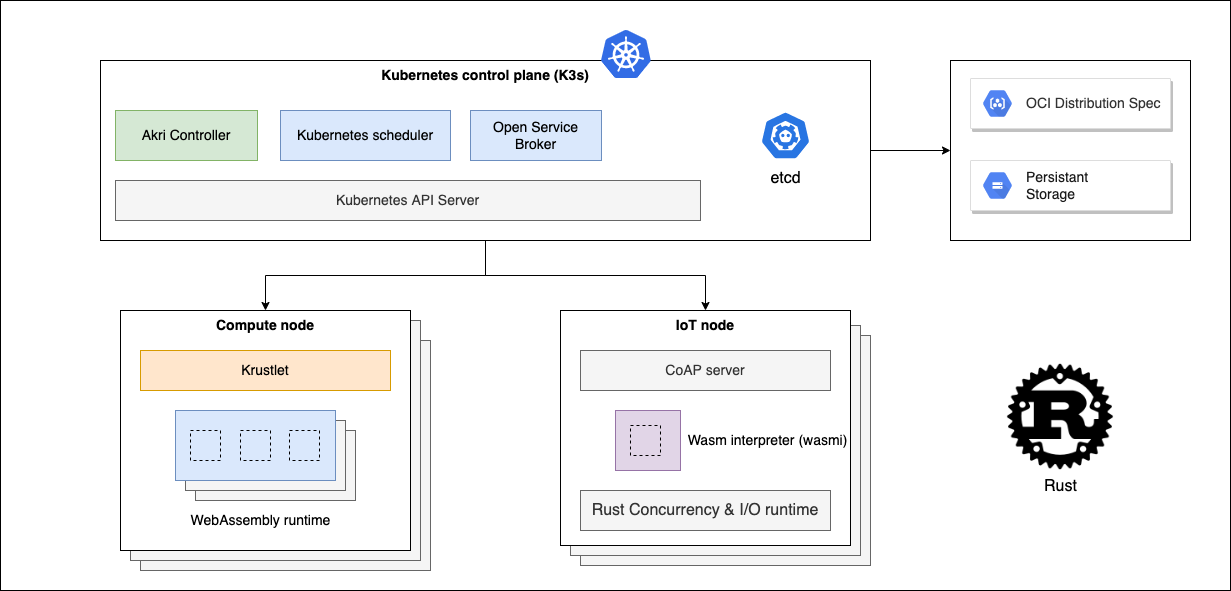
\includegraphics[width=\columnwidth]{figures/architecture-technologies}
\caption{Technology baseline for the reference infrastructure architecture.} \label{fig:architecture-technologies}
\end{figure}

We briefly also revisit our previous system for weather-based service as a representative of how the above technologies can be used in synergy:

\begin{itemize}
    \item Sensor nodes: the arbitrary code execution is safely enabled by running a Rust-based WebAssembly interpreter on the Wasm binary file. The portable low-overhead Wasm format unlocks transfer of computation to dynamically instruct the sensor nodes about the preprocessing logic on a case-by-case basis;
    \item Broker nodes: brokers subscribe to the sensor nodes, which expose their data as REST resources via CoAP messages, and the devices periodically send CoAP updates. In turn, the brokers forward them to the cluster as WebSocket packets. The broker ensures that both parts, IoT nodes and services nodes, are independent as they agree to communicate following the REST architecture. Service nodes typically use REST over HTTP, while sensor nodes prefer CoAP;
    \item Service nodes: they request the weather information as services to the service platform implementing the Open Service Broker API. The latter also exposes conventional services like storage, offering both locally provided solutions and Cloud-based alternatives on Google Cloud under the same RESTful interface. 
\end{itemize}

\section{WebAssembly analysis}\label{sec:wasm}

\subsection{Rationale and devices}

We now proceed with an in-depth analysis of WebAssembly. WebAssembly is the common denominator of several challenges, notably portability and virtualization, that in turn will enable other key characteristics of the Continuum like computational mobility. As such, for this work, we decided to focus our extensive evaluation on this topic alone.

For the evaluation, we have used the following devices:

\begin{itemize}
    \item Edge cluster nodes: 4 Raspberry Pi 4 Model 3B+ with Quad-core Cortex-A53 (ARMv8) 64-bit SoC at 1.4GHz and 1 GB physical memory. The Raspberry 3B+ model has been chosen to showcase the feasibility of the presented technologies on limited low-powered machines, relatively cheap and with only 1GB of memory. This offers results comparable with other researches regarding containerised virtualization over Raspberry Pi \cite{bellavista2017feasibility};
    \item Sensor nodes: STM32F407 microcontrollers with ARM Cortex-M4 core, 512KiB flash storage, and 128KiB of memory. The device is also capable of many 32-bit floating-point operations.
\end{itemize}

Raspberry Pi and STM32F407 microcontrollers are designed for moderately high computational performance, low unit cost, and power efficiency in Edge and IoT computing environments. We trust these empirical results generalise to other ARM machines and microcontrollers in the Cortex-M family.

\subsection{Wasm for IoT devices}

\begin{figure}[ht]
\centering
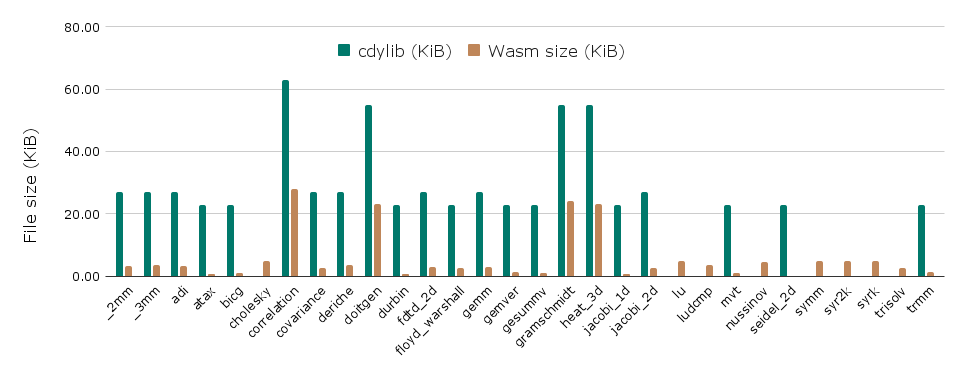
\includegraphics[width=\columnwidth]{figures/b-wasmi-3}
\caption{Comparison of Wasm size (KiB) and C dynamic library size (KiB).} \label{fig:b-wasmi-3}
\end{figure}

Figure~\ref{fig:b-wasmi-3} presents a comparison of the sizes of different Wasm binaries compiled from the Polybench~\cite{yuki2014understanding} modules. The Polybench benchmark suite offers relevant functions to embedded systems as it includes common matrix and statistical operations. We have chosen the C dynamic library size as a meaningful comparison since it is a close alternative to Wasm binary files. Both outputs have been compiled from the same Rust source code and using the same LLVM toolchain and optimisation flags.

The results undeniably favour the Wasm binary format as the C dynamic lib is often many times larger. Comparing Wasm files to containers would be even less relevant and greatly favour the former, as containers package a whole operative system filesystem, unnecessary for pure computational IoT services. Even the tiniest image base (Alpine Linux Mini Root Filesystem) has an additional size of about 5.5MB uncompressed.

\begin{figure}[ht]
\centering
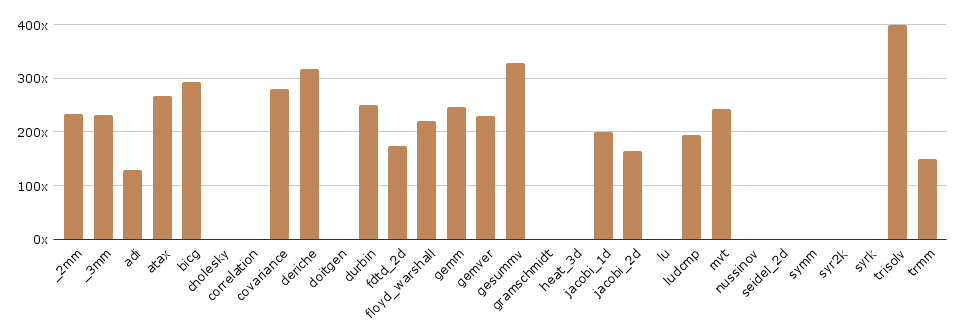
\includegraphics[width=\columnwidth]{figures/b-wasmi-4}
\caption{Comparison of Wasm interpreter performance and Rust native performance.} \label{fig:b-wasmi-4}
\end{figure}

Figure~\ref{fig:b-wasmi-4} plots the slowdown of the Wasm interpreter executing Polybench benchmarks on the STM32F407 microcontroller against native Rust. The results show a dramatic slowdown, with a factor of 100-400X. Such results dispel the notion of using Wasm interpreters on microcontrollers to support dynamic reconfiguration.
However, it is fair to say that the Wasm interpreter we used, wasmi~\cite{wasmi}, was the only available Rust WebAssembly interpreter and we adapted it to work on embedded devices. The interpreter was designed for safe execution in the blockchain instead of efficiency in highly constrained devices. 
% Wasmi is developed for blockchain execution; as such it is used to offer a deterministic sandboxed execution context running on Cloud servers. Accordingly, embedded execution performance is not paramount to it, unfortunately.
Alternative embeddable interpreters, implemented in the memory-unsafe C language, shows a much inferior execution penalty, in the order of 30-60x slower than native~\cite{peach2020ewasm}. Arguably, however, a 30x execution penalty can still seriously deter the usage of interpreters in microcontrollers.

% \begin{figure}[ht]
% \centering
% 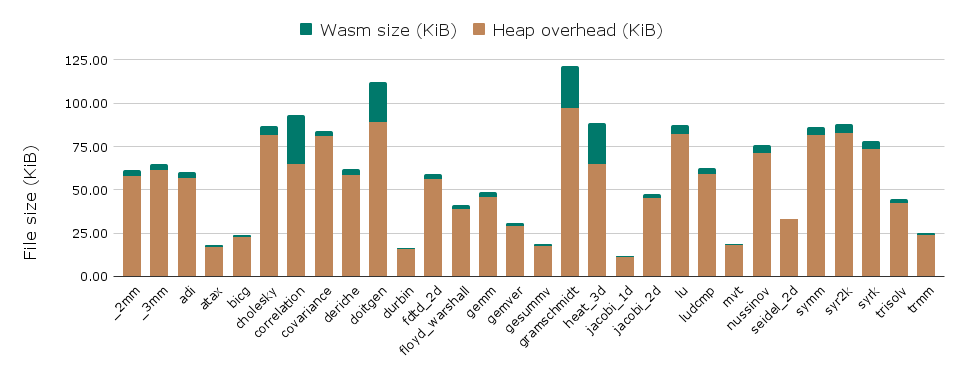
\includegraphics[width=\columnwidth]{figures/b-wasmi-1}
% \caption{Comparison of Wasm size (KiB) and heap overhead (KiB).}
% \label{fig:b-wasmi-1}
% \end{figure}

% We have evaluated the heap overhead of interpreting Wasm on microcontrollers as an additional benchmark. 
% Figure~\ref{fig:b-wasmi-1} presents a significant increase in the heap usage with respect to the Wasm size.

Another crucial concern we have found in our work is that the heap overhead of using Wasm interpreters is not predictable. Such unpredictability does not come again in favour of the usage of WebAssembly on microcontrollers, as embedded devices have extremely limited resources and must have predictable behaviours to ensure proper execution. Such deficiency is an intrinsic issue with interpreters, as the code instructions and execution data structures must be stored in heap memory. This behaviour contrasts with the binary executables that can save and access instructions or read-only data on the more capable flash storage. Writable data is saved in the stack instead, and it can be estimated with accuracy in many production-grade toolchains like C and Ada.

Finally, running Wasm on resource-constrained microcontrollers also presents a memory-design issue. Wasm's pages are 64KiB by standard, too large for microcontrollers that often have between 16-256 KiB RAM. Dynamic allocation is a common requirement even for embedded systems. However, Wasm specifies that the sandbox should expand memory by 64KiB chunks, insufficiently granular for constrained embedded systems. Consequently, we had to adapt the interpreter to allocate non-standard pages of 16KiB. Otherwise, it would have been impossible to execute any benchmark on the STM32F407 microcontroller, as additional heap space is required for the interpreter's internal structures and the Wasm instructions themselves.

\subsection{Wasm on the Cloud}

We successfully integrated WebAssembly into Kubernetes with Wasm Pods running on Krustlet~\cite{krustlet}, while the container Pods are scheduled on K3s~\cite{k3s} Kubelet. Krustlet (a Kubernetes-Rust-Kubelet stack) is an experimental implementation of the Kubernetes compute node (Kubelet) API that supports Wasm as virtualisation technology. Therefore, it listens to the Kubernetes API event stream for new units of execution (Pods) and runs them under a WebAssembly System Interface (WASI) runtime (notably, Mozilla's Wasmtime~\cite{wasmtime}).

K3s is a fully certified Kubernetes distribution geared towards Edge environments backed by a commercial company. K3s is implemented in Go and packaged as a single binary of about 50MB in size.
% It bundles everything needed to run Kubernetes, notably the container runtime containerd~\cite{containerd}.

At the time of writing, it has not been however possible to implement a portable web server (e.g. to act as an electrical load forecasting service) and compile the application to Wasm. There is an underlying issue with implementing network servers as there is neither sufficient network API nor multi-threading support in the standard yet.

On the one hand, the current WebAssembly System Interface (WASI) standard only contains a few methods for working with sockets that are not enough for complete networking support. Adding support for connecting to sockets is fundamental to allow Wasm modules to connect to web servers, databases, or any service. \\
On the other hand, the lack of concurrency primitives means that a server running in WebAssembly is single-threaded, or its implementation has to be significantly more complex (e.g. Node.js's event loop~\cite{nodejs-event-loop}). This limitation severely limits the workload capabilities of the server. Lately, the WebAssembly specifications have outlined a thread and atomics proposal intending to speed up multi-threaded applications. At this time of this writing, that proposal is still in the early stage, and it is implemented only in web browsers, behind an experimental flag.

% In the field of machine learning, numerical precision matters. WASM natively supports floating-point arithmetic, whereas other popular machine learning backends like WebGL requires hardware extensions. Not all devices support this extension, which means a GPU-accelerated machine learning is not supported on some devices (e.g. older mobile devices which can run Wasm instead).

% Moreover, GPU drivers can be hardware-specific and different devices can have precision problems. In WASM, computation always happens in 32-bit floats and thus have precision parity across all devices. Such numerical predictability is also paramount in blockchain applications \textcolor{red}{, as proved by Parity's interest in WebAssembly}~\cite{parity-wasm}.

Finally, it is also worth mentioning that the weather-based flood prediction model that we compiled to Wasm is a conventional Deep Neural Network. The modal is constituted by dense layers trained on the Cloud using the traditional machine learning framework Keras~\cite{keras}. As of the time of writing, TensorFlow~\cite{tensorflow} provides a WebAssembly backend only for the browser and Node.js~\cite{tf-wasm}. As a result, the model is saved to the alternative ONNX~\cite{onnx} standard format and executed by a WebAssembly neural network inference library (\emph{tract}~\cite{tract}) that can read and run Tensorflow or ONNX models. \\

% We tested the feasibility of employing WebAssembly in our PoC by measuring several metrics: how long it takes to create and boot a Wasm-based Kubernetes Pod, how memory scales as the number of running Pods increases, and how both metrics compare to containers. The benchmark is a simple DateTime application that logs the current system time upon creation and goes into sleep. The Pod does not complete by going to sleep, and the resources remain allocated. The log is later retrieved using the Kubernetes API to calculate the boot time. 

% \begin{figure}[ht]
% \centering
% 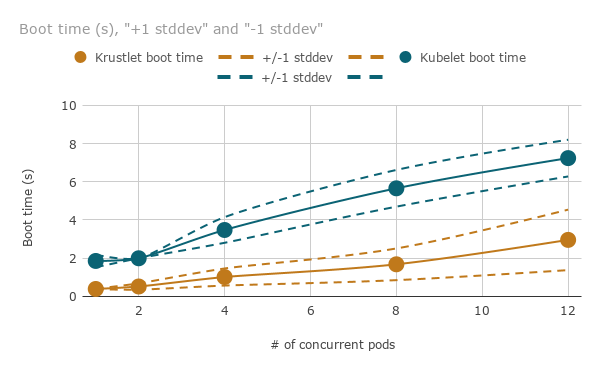
\includegraphics[width=\columnwidth]{figures/b-krustlet-1}
% \caption{Average boot time for concurrent Wasm Pods.}
% \label{fig:b-krustlet-1}
% \end{figure}

% Figure~\ref{fig:b-krustlet-1} shows the average boot time, along with the standard deviation, of both the Kubernetes Pods containing Wasm binaries and the conventional Pods containing containers. The benchmark concurrently deploys the Pods and repeats the process 15 times. Pods are not deleted between iterations so that increasing memory utilisation is also collected.

% The experimental results show that a Wasm-based virtualisation strategy incurs less boot time. However, there is no clear winner because efficient concurrency is essential as much as fast boot time. Nevertheless, such preliminary results encourage the idea of adopting Wasm as an alternative to container technology since efficiency was not a primary design goal in the early implementations of Krustlet and Wasmtime. We expect future versions will provide even more competitive results.

% \begin{figure}[ht]
% \centering
% 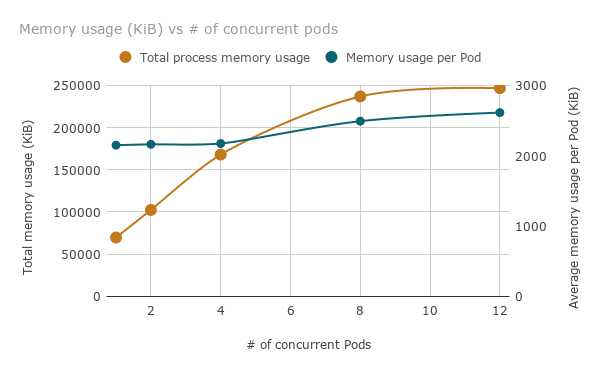
\includegraphics[width=\columnwidth]{figures/b-krustlet-2}
% \caption{Average memory usage of concurrent Wasm Pods.}
% \label{fig:b-krustlet-2}
% \end{figure}

% \begin{figure}[ht]
% \centering
% 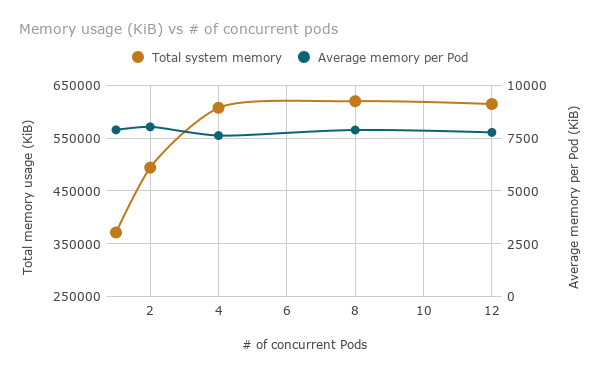
\includegraphics[width=\columnwidth]{figures/b-krustlet-3}
% \caption{Average memory usage of concurrent K3s Kubelet Pods.}
% \label{fig:b-krustlet-3}
% \end{figure}

% Figures~\ref{fig:b-krustlet-2} and~\ref{fig:b-krustlet-3} offer an overview of the memory overhead of the two different virtualisation solutions. In such a comparison, Wasm Pods are the winners in memory usage per unit, but K3s Kubelet can achieve higher total memory utilisation. Notably, K3s Kubelet may use up all available memory until the machine becomes unable to function properly. Conversely, the Krustlet node fails to allocate new Pods even with sufficient memory space. The allocation results in an Out Of Memory error because of Rust's default allocation strategy, but the node is still completely functional.

% On a different note, as Go is a garbage-collected language, heap utilisation is known to be highly unpredictable. Besides, as the GC kicks in only when the heap size doubles, memory is underutilised. The freeable memory should be used for running additional Pods, achieving better Pod packing. Such efficiency is crucial for Edge nodes that have already limited hardware capabilities but must support multiple workloads. This consideration is another point in favor of adopting Rust. Table \ref{tab1} reports the system memory utilised by an idling node.

% Finally, the memory overhead per Pod is relatively constant in both technologies. However, the Wasm Pod incurs approximately 2x-3x less overhead, which allows more efficient packing of applications on the same machine. Another significant difference is that Krustlet does not allocate more Wasm Pods when the limit is reached, but existing Pods are still completely functional. 
% Conversely, the K3s Kubelet makes the entire node completely unresponsive when maximum memory utilisation is reached. Arguably, such results warrant favouring Krustlet, as the premature Out Of Memory error is likely to be fixed by future Wasmtime versions.
% This room for further improvement contrasts with the container overhead, which is at the state of the art of a decade of research in container technologies.

% \begin{table}\label{tab:k3s-memory-usage}
% \caption{Memory usage of Kubernetes on Edge Raspberry Pi.}
% \begin{tabular}{|l|l|}
% \hline
% Software stack & Idle memory usage \\
% \hline
% Alpine Linux 3.12.1 & ~50MB \\
% Alpine Linux + K3s master & ~304MB \\
% Alpine Linux + K3s agent & ~110MB \\
% Alpine Linux + Krustlet & ~120MB \\
% \hline
% \end{tabular}
% \label{tab1}
% \end{table}

% \subsection{Evaluation of CoAP for microcontrollers}

% \begin{figure}[ht]
% \centering
% 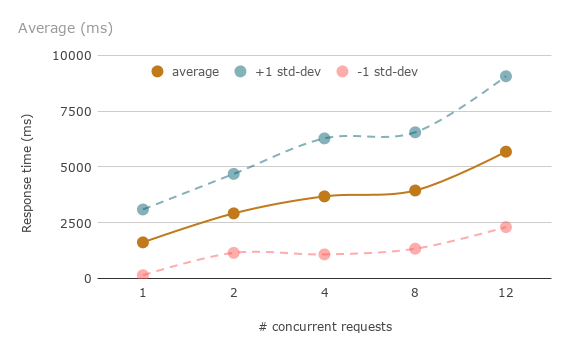
\includegraphics[width=\columnwidth]{figures/b-coap-1}
% \caption{Average response time for concurrent CoAP requests \label{fig:b-coap-1}}
% \end{figure}

% \begin{figure}[ht]
% \centering
% 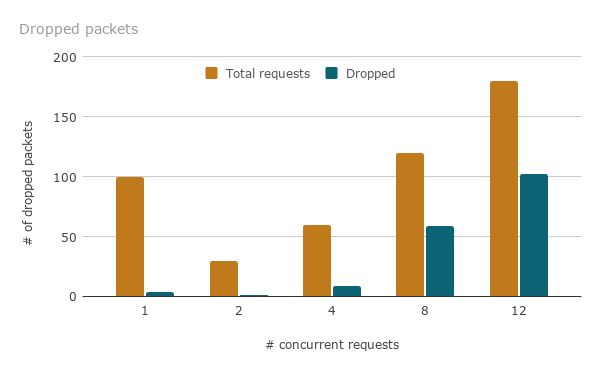
\includegraphics[width=\columnwidth]{figures/b-coap-2}
% \caption{Number of dropped packets as concurrency increases \label{fig:b-coap-2}}
% \end{figure}

% Fig. \ref{fig:b-coap-1} and Fig. \ref{fig:b-coap-2} present the experimental evaluation of the CoAP implementation in Rust. The STM32F407 is equipped with a LAN8720 ETH 10/100Mbs module connected to the microcontroller via cheap jumper wires. On the software stack, the device offers a CoAP server running on the RTIC runtime. Such a server is put under stress by firing concurrent requests from a machine connected to the same network, and the test is repeated 15 times. As expected, the response times increase as the number of concurrent requests rises. However, such escalation of response time is not exponential and presents a good smoother curve. The standard deviation range is also significantly large, as the embedded device cannot provide timely responses. Further experiments should compare the CoAP server with an equivalent HTTP or MQTT server running on the same RTIC runtime.

% On a different note, the number of dropped packets dramatically increases as the concurrency grows. Such behaviour is expected, and the experimental logs provide a plausible rationale. As the number of concurrent requests increases, the microcontroller network buffers cannot cope with the volume, and the packets are even truncated before being parsed. A deeper analysis should check whether the issue can be solved by allocating more buffer space or, on the contrary, is a hardware-related limit. Admittedly, the hardware network connection via jumper wires is not the most robust solution.

To summarise the current state of WebAssembly, the technology overall design is highly promising for the fits of the Continuum. In practice, the current standard and, subsequently, the industry implementations, severely limit the feasibility of applications that can be deployed on constrained and relatively powerful machines alike. The underlying theme is that the Wasm specifications (notably memory management, networking and concurrency) are not mature or robust enough for real-world application, let alone innovative Continuum services. At the time of writing, it is still the application developer's responsibility to concretely navigate the WebAssembly landscape, leading them to create ad-hoc workarounds~\cite{wasm-experimental-http} and hindering portability.

\section{Conclusion}
\label{sec:conclusion}

In this paper we have presented a Continuum of Computing constituted by software and hardware resources provided as a service and delivered anywhere the user is, independently of their respective location. 
In the intent of evaluating its viability for real-world industrial applications, we uncovered the difficult challenges that the research community will have to face to make the Continuum real. 
%Admittedly, none of such challenges is easy to solve, and the current state of the candidate technologies is a perfect portrait of such hardship.

For many of such challenges, we have shown that present-day technologies align well in principle with the envisioned needs of the Continuum, but they are still very far from sufficient maturity for industrial use.

% Projects like Akri for Kubernetes still are in their infancy and rated as explorative by some of the major players in the Cloud industry, notably Microsoft and Huawei. Even relatively well-adopted standards like the Open Service Broker API are still incapable of solving common problems that different stakeholders are facing, such as managing the lifecycle of chains of service dependencies.

The experience reported in this paper allows us to conclude that many solutions needed by the Continuum are organically sprouting in the areas of Cloud and Edge development, which is very encouraging. Problems like IoT orchestration, service composition and multi-platform virtualisation are prominent hot challenges. Naturally, each of them has attracted interest in the last few years and nascent solutions have emerged consequently, but we have not observed any underlying governance over the evolution of these areas.

Our empirical results show that present WebAssembly is nearly exclusively suited for pure compute functions, which is a natural fit for the Serverless but too restricting for the Continuum. The lack of multi-threading and a mature network interface severely limit the space of real-world applications that WebAssembly can serve.
Likewise, the results we obtained from running WebAssembly on microcontrollers discourage the idea of using its interpreters on resource-constrained nodes. On the bright side, however, we trust these problems should be overcome given sufficient time and effort by the developers' community. On this account, we anticipate WebAssembly to receive significant attention in the coming years.

% \paragraph{Mobility}
% In the Continuum, services should be relocated following the user's movements, and so should the corresponding data and state. 
% It, therefore, follows that all synchronisation, data \& state migration, handshakes and collaboration needs have to be addressed across multiple layers of the compute and communication infrastructure.
% When mobility is involved, provisioning data and services should be highly reactive and reliable, which is a challenge. 
% For example, present-day vehicular networking and communication reportedly appear to be intermittent or unreliable \textcolor{red}{\cite{he2014developing}}.

% \paragraph{Security and Privacy}

% The seamless integration of Edge and Cloud computing is bound to raise unforeseen security issues. Previously unexplored scenarios, such as the interplay of heterogeneous Edge nodes and the migration of services across global and local scales, create the potential for original channels of malicious behaviour~\cite{yu2017survey}.

% In point of principle, end-user data originated at the Edge should be stored locally, with the user able to control whether and which service providers be allowed to access them. 
% As long as Edge nodes expose vulnerabilities (e.g. tampering, spoofing, falsifying), however, storing and processing privacy-sensitive data there should be regarded as far more hazardous than retreating them at the centre of the Cloud.
